We report our investigation of the dynamics of a colloidal particle in a Prandtl-Tomlinson setup, focusing on the effects of a non-Markovian environment. To make contact with Ref.\cite{ginot2022}, we begin our analysis by examining the dynamics of barrier crossing and the distributions of waiting times of the colloidal particle in a minimum. We conduct separate comparisons between pure, no driving, jump-diffusion with and without memory effects, as well as between the complete Prandtl-Tomlinson model and its non-Markovian extension. Finally, we compare the velocity-dependent behavior of the friction force between the standard PT model and its non-Markovian version.
\section{Effective potential}
In this section, we aim to begin understanding how a viscoelastic environment influences the motion of a colloidal particle threading a sinusoidal energy landscape. To achieve this, we first address the effective potential to which the particle is subjected in Brownian motion and its extension within a non-Markovian environment.

In these conditions, characterized by purely thermal effects, the probability distribution of the positions of a particle follows the Boltzmann equilibrium probability distribution.
\begin{equation}
    P(x) = \dfrac{1}{Z} e^{-\beta V_\text{eff}(x)}\, ,
\end{equation}
here $x$ denotes the position, $V_\text{eff}(x)$ the effective potential energy acting on the particle, $Z$ represents the partition function and $\beta =(k_B T)^{-1}$.
From this relation, we can express the effective potential as follows
\begin{equation}
    V_\text{eff}(x)=-k_BT \left(\log{Z} + \log{P(x)}\right)\, .
    \label{eq:potenz_efficace}
\end{equation}
Here the partition function $Z$ contributes just an irrelevant additive constant.
\begin{figure}
    \centering
    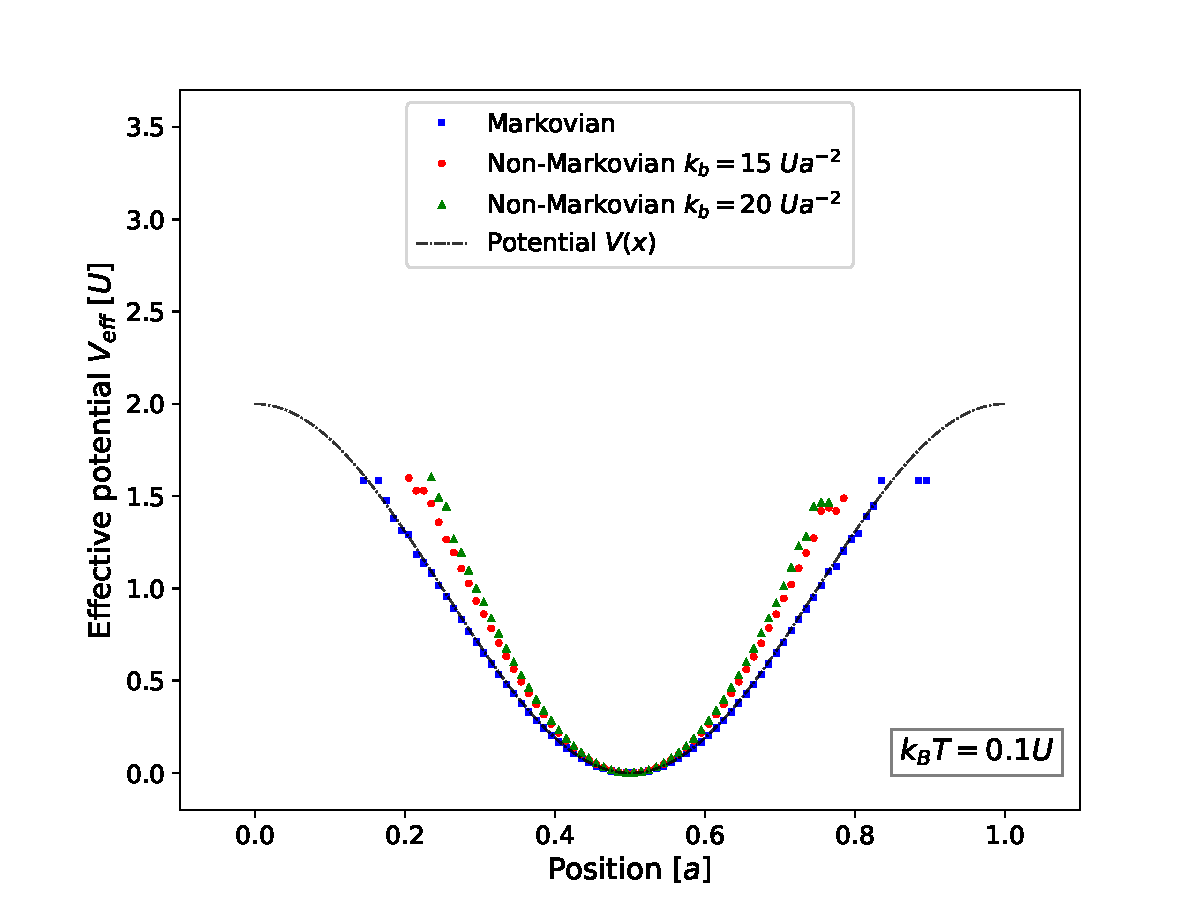
\includegraphics[width=\textwidth]{T01_U_eff.pdf}
    \caption{Comparison of the effective potential $V_\text{eff}(x)$ obtained through a histogram of the successive positions along a simulation at $k_BT=0.1\hspace{0.1cm}U$ through Eq.\eqref{eq:potenz_efficace}, for the standard Markovian environment ($k_b=0$) and two values of couplings $k_b$ to the memory bath. The actual potential, shifted so that its minimum coincides with the $k_b=0$ curve, is also shown as a dot-dashed line for comparison.}
    \label{fig:eff_pot_kbt01}
\end{figure}
To evaluate the probability distribution of the particle positions $P(x)$ we wrote a python script which maps the particle's position at successive simulation steps onto $0\leq x \leq 1\hspace{0.1cm}a$ of the corrugation potential and evaluate a 100-bins histogram of position occurences along the simulation. From the resulting normalized histogram, using relation \eqref{eq:potenz_efficace}, we reconstruct a map of the effective potential $V(x)$ experienced by the Brownian particle. Figure \ref{fig:eff_pot_kbt01} reports the resulting effective potential for the standard Markovian environment, and for 2 values of the coupling spring to the non-Markovian bath, evaluated for $k_BT=0.1\hspace{0.1cm}U$. At this low temperature, the Boltzmann factor at the maxima is $e^{-20} \simeq 2 \cdot 10^{-9}$ times smaller than at the minima, so even though the simulation cover $N=10^9$ steps, in practice the maxima are never explored, and this figure covers just the low-energy region near the minimum. Even with this drawback, it is apparent that in the presence of the non-Markovian thermostat, the effective potential experienced by the particle is steeper. We have also explored $k_BT=0.2\hspace{0.1cm}U$. At this higher temperature the regular Markovian bath has a relative Boltzmann probability of visiting the maximum that is $e^{-10} \simeq 4.5 \cdot 10^{-5}$ smaller than that of sitting at a minimum. In this condition, indeed, the Brownian particle is able to explore all the points of the potential, occasionally reaching the maxima in simulations of $10^9$ steps. However, this practically never occurs in the presence of a non-Markovian environment. For this reason, we raise the temperature to $k_BT=0.5\hspace{0.1cm}U$, allowing the model to explore the maxima of the potential a sufficient number of times for accumulating a significant statistics. 
\begin{figure}[ht!]
    \centering
    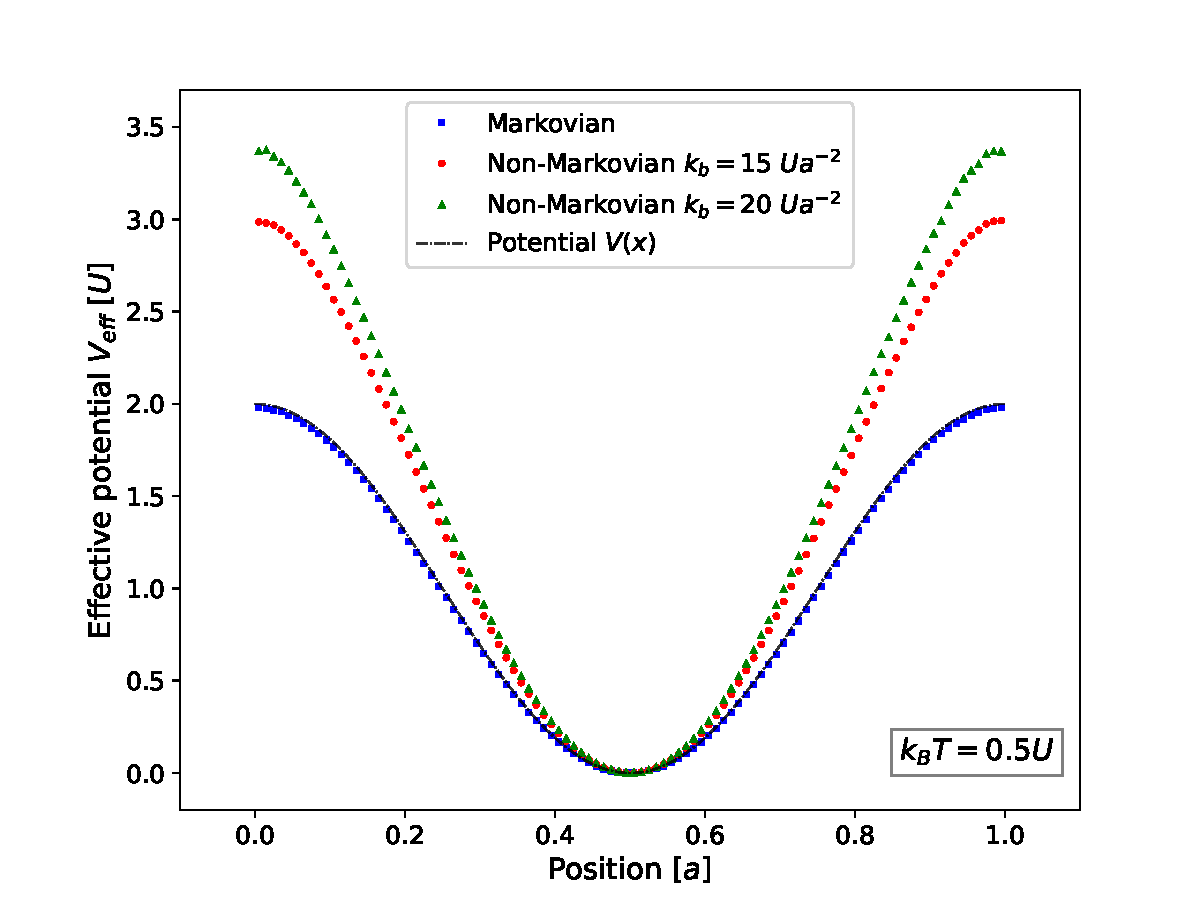
\includegraphics[width=\textwidth]{T05_U_eff.pdf}
    \caption{Same as Fig. \ref{fig:eff_pot_kbt01}, but for a substantially higher $k_BT=0.5\hspace{0.1cm}U$}
    \label{fig:effpotenz}
\end{figure}
\\
Figure \ref{fig:effpotenz} perfectly illustrates that for a simple Brownian particle, the effective potential $V_\text{eff}(x)$ coincides exactly with the corrugated potential on which it moves. Furthermore, it is observed that the effect of the viscoelastic non-Markovian environment is to raise the potential barrier while leaving the position of the minimum unchanged at $x=0.5\hspace{0.1cm}a$, thus making it much steeper. These simulations are carried out for $10^9$ time steps to ensure a sufficient number of counts in each bin, thus correctly sampling the effective potentials $V_\text{eff}(x)$.
\section{Waiting-time distribution}
To gain deeper insights into the motion of a colloidal particle across a viscoelastic bath in this section we investigate the barrier-crossing dynamics of a particle under various conditions. Initially we are going to study the dynamics of barrier crossing under pure Brownian non-driven conditions, followed by a study of this statistics for the full Prandt-Tomlinson model. 
\begin{figure}[ht!]
    \centering
    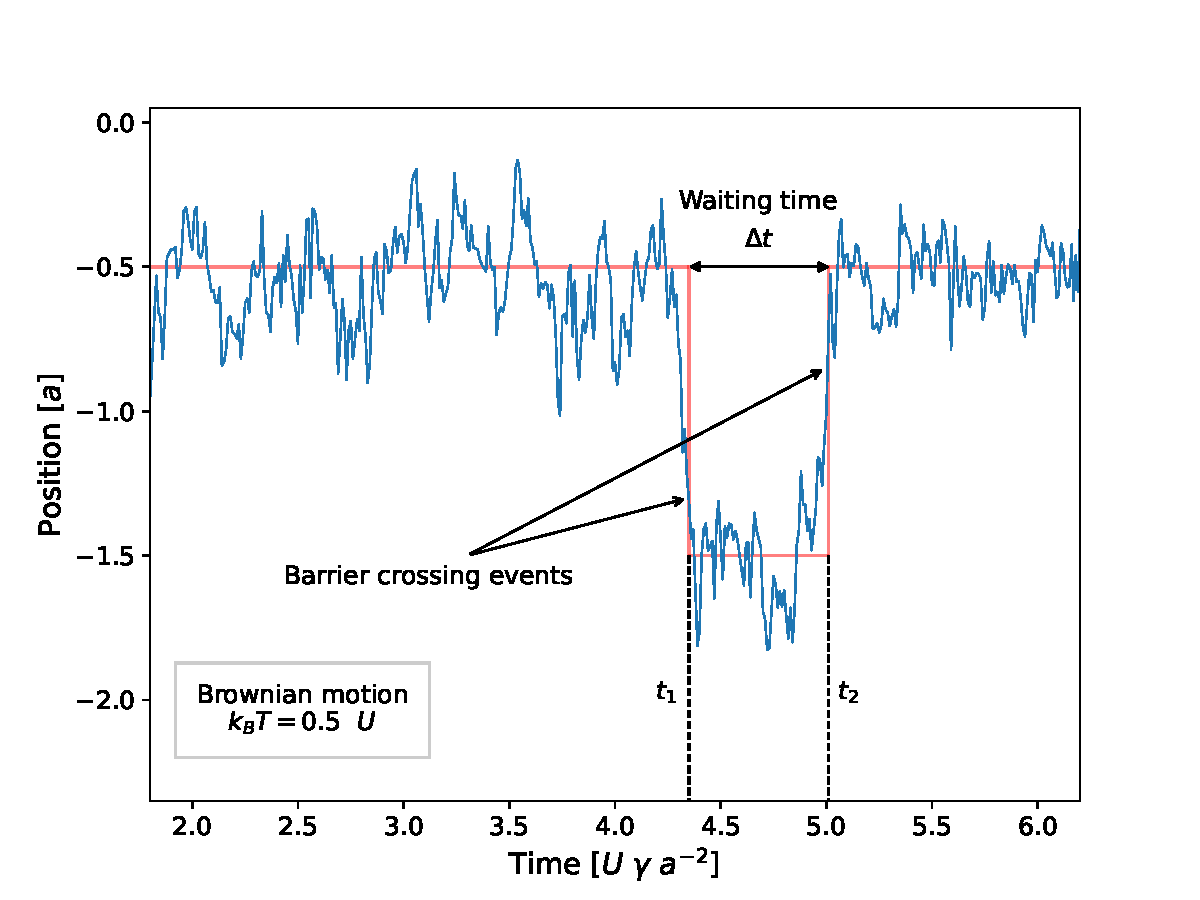
\includegraphics[width=\textwidth]{definition_barrcross2.pdf}
    \caption{Visual definition of barrier crossing event and waiting time}
    \label{fig:definition_barrcross}
\end{figure}
\\
Firstly, let us define a barrier-crossing event as the instant when the particle's displacement reaches at least $x = 0.7 \hspace{0.1cm}a$ from the current minimum.
This condition assures us that the colloidal particle definitely left the minimum and has transitioned into one of the adjacent minima. Moreover we define the waiting time as the duration between two consecutive crossing events, see Fig.~\ref{fig:definition_barrcross}.
To analyze barrier-crossing events and waiting times we have developed a python code to calculate the probability distribution $P(t_\text{w})$ of waiting times $t_\text{w}$ in the minima. This probability distribution $P(t_\text{w})$ is developed through a histogram characterized by a variable bin width allowing us to capture a fair detail of the short timescale and to ensure an adequate number of points to produce a fair statistics of long waiting times. The histogram is adequately normalized to $1$ to allow a fair comparison of different trends, in a correctly-normalized probability density.
\subsection{Brownian motion and non-Markovianity}\label{sec_markov_vs_non}
In this part we compare simple Brownian diffusion with diffusion in a viscoelastic bath. As previously explained, Brownian diffusion characterises the stochastic movement of a particle suspended in a fluid due only to time-independent memory-free effects and collisions with surrounding particles of the fluid. When the surrounding medium is a viscoelastic fluid, the environment generates memory effects keeping track of previous particle positions.

Figure \ref{P_kb15} shows a comparison between the probability distributions of waiting times $P(t_\text{w})$ of simple Brownian diffusion ($k_b=0$, triangles) and $P(t_\text{w})$ in the non-Markovian environment simulated with $k_b=15\hspace{0.1cm}Ua^{-2}$ (squares). For these simulations we consider $k_BT=0.5 \hspace{0.1cm}U$.
\begin{figure}[h!]
    \centering
    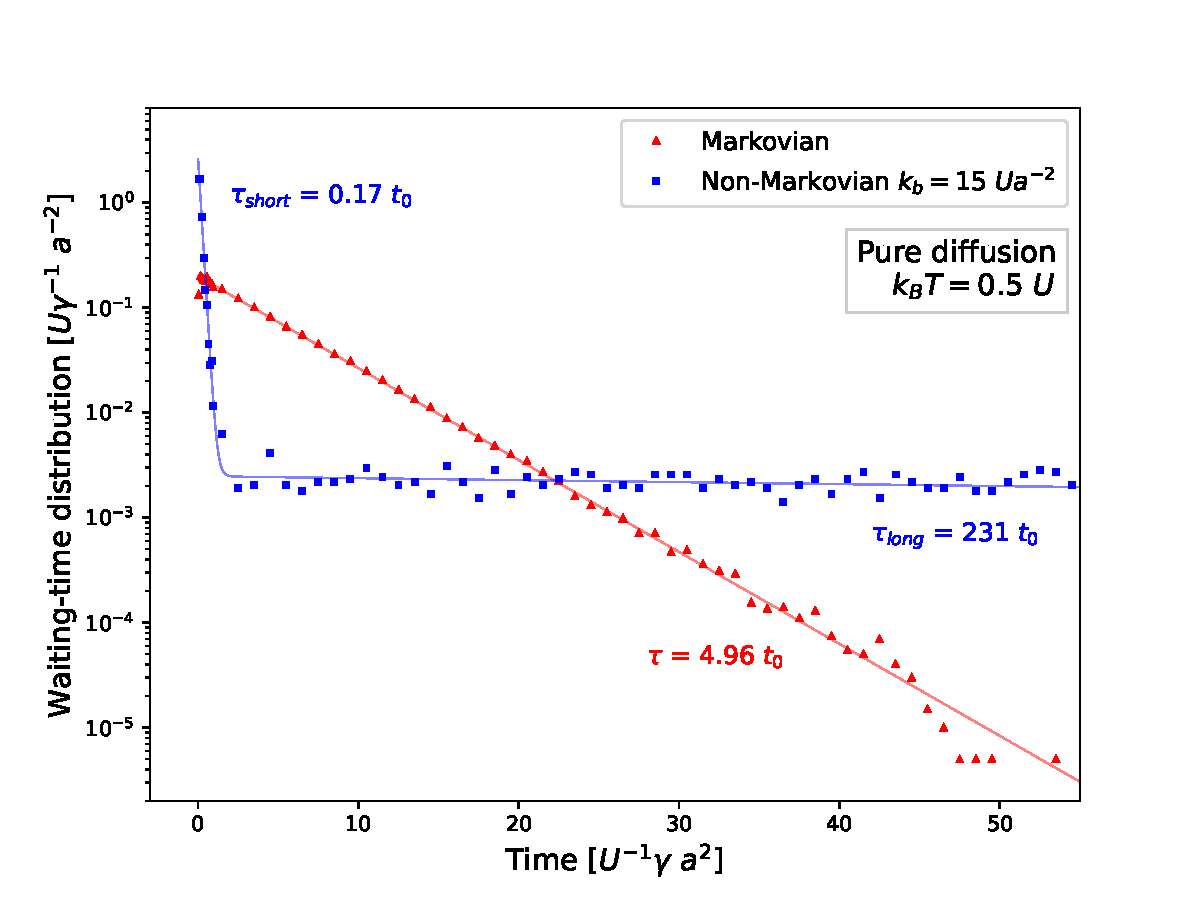
\includegraphics[width=\textwidth]{kb15_T05.pdf}
    \caption{Comparison of the waiting-time distributions of a simple Brownian particle and the same particle in a non-Markovian environment ($k_b=15\hspace{0.1cm}Ua^{-2}$), both simulated at $k_BT = 0.5\hspace{0.1cm}U$}
    \label{P_kb15}
\end{figure}
\\
In Figure \ref{P_kb15} the histograms are characterized by a variable bin width: $0.1\hspace{0.1cm}t_0$ from $0$ to $1$ and $1\hspace{0.1cm}t_0$ from $1$ to $100$.
\\
As suggested by the lin-log scale, the probability distribution of waiting times in the ordinary Markovian environment $P_{k_b=0}(t_\text{w})$ follows an exponential decay in the form 
\begin{equation}
    P_{k_b=0}(t_\text{w})= A \exp{\left(- \dfrac{t_\text{w}}{\tau}\right)}\,.
    \label{eq:P_kb0}
\end{equation}
The solid line in Fig. \ref{P_kb15} is a fit of the histogram points, obtained using an appropriate NumPy function. Table \ref{tab:fit_brownian_diffusion} presents the best fit parameters $A$ and $\tau$.
\begin{table}[ht]
\centering 
\begin{tabular}{cc}
    \toprule
    Parameter & Value  \\
    \midrule 
    $\tau \hspace{0.1cm} [t_0]$ & $4.96\pm 0.05$ \\[0.5ex]
    $A \hspace{0.1cm} [t_0^{-1}]$ & $0.20\pm 0.01$ \\
    \bottomrule
\end{tabular}
\caption{Best fit parameters of the waiting-time distribution $P(t_\text{w})$, Eq.\eqref{eq:P_kb0}, for the standard, Markovian thermostat inducing Brownian diffusion.}
\label{tab:fit_brownian_diffusion}
\end{table}
\\
\noindent The waiting-time statistics for the Brownian particle with memory is remarkably different: Figure \ref{P_kb15} shows that the probability distribution exhibits a double exponential decay with two different time scales: a short timescale associated to back-and-forth events with the particle being recalled into the originating minimum shortly after the jump due to viscoelastic effects, and a long timescale corresponding to regular diffusive processes. To evaluate the relative time scales, we decide to lead us to fit the delay times with the sum of two exponential decays in the following form:
\begin{equation}
    P(t_\text{w}) = A_\text{short} \exp{\left(- \dfrac{t_\text{w}}{\tau_\text{short}}\right)} + A_\text{long} \exp{\left(- \dfrac{t_\text{w}}{\tau_\text{long}}\right)}\,.
\end{equation}
Table \ref{tab:fit_brownian_withmemory} reports the coefficients obtained and the associated errors.
\begin{table}
\centering 
\begin{tabular}{ccc}
    \toprule
    Fit parameter & $k_b=15\hspace{0.1cm}[Ua^{-2}]$& $k_b=20\hspace{0.1cm}[Ua^{-2}]$\\
    \midrule 
    $\tau_\text{short} \hspace{0.1cm} [t_0]$ & $0.17\pm 0.01$ & $0.13 \pm 0.01$\\[0.5ex]
    $A_\text{short} \hspace{0.1cm} [t_0^{-1}]$ & $2.6 \pm 0.4$ & $0.0012 \pm 0.0001$\\[0.5ex]
    $\tau_\text{long} \hspace{0.25cm} [t_0]$ & $231 \pm 12$ & $460 \pm 93$\\[0.5ex]
    $A_\text{long} \hspace{0.2cm} [t_0^{-1}]$ & $ 0.0025 \pm 0.0001$ & $5 \pm 2$\\
    \bottomrule
\end{tabular}
\caption{Parameters of waiting-time distributions $P(t_\text{w})$ for Brownian diffusion with memory effects of Figs. \ref{P_kb15} 
 ($k_b=15\hspace{0.1cm}Ua^{-2}$) and \ref{P_kb20} 
 ($k_b=20\hspace{0.1cm}Ua^{-2}$), both simulated at $k_BT=0.5\hspace{0.1cm}U$ }
\label{tab:fit_brownian_withmemory}
\end{table}
\\
Figure \ref{P_kb20} reports similar results for a stiffer viscoelastic thermostat ($k_b=20\hspace{0.1cm}Ua^{-2}$). Comparing Figs. \ref{P_kb15} and \ref{P_kb20}, we can observe how the viscoelastic bath, and thus the memory of the environment, influences the distribution of waiting times in the potential minima. In particular, we observe that the Brownian motion with memory supports even very long waiting times of hundreds of time units, as opposed to the regular Markovian thermostat, for which long waiting times in excess of a few tens of time units are radically suppressed at the explored temperature. In the short-times region, the viscoelastic rapid-recall mechanism has the distribution of non-Markovian waiting times exceed that of the regular Markovian bath. In contrast, in the $0.3\hspace{0.1cm}t_0 \lesssim t_\text{w} \lesssim t_0$ range, the regular Markovian dynamics leads to more likely delay times.
\begin{figure}
    \centering
    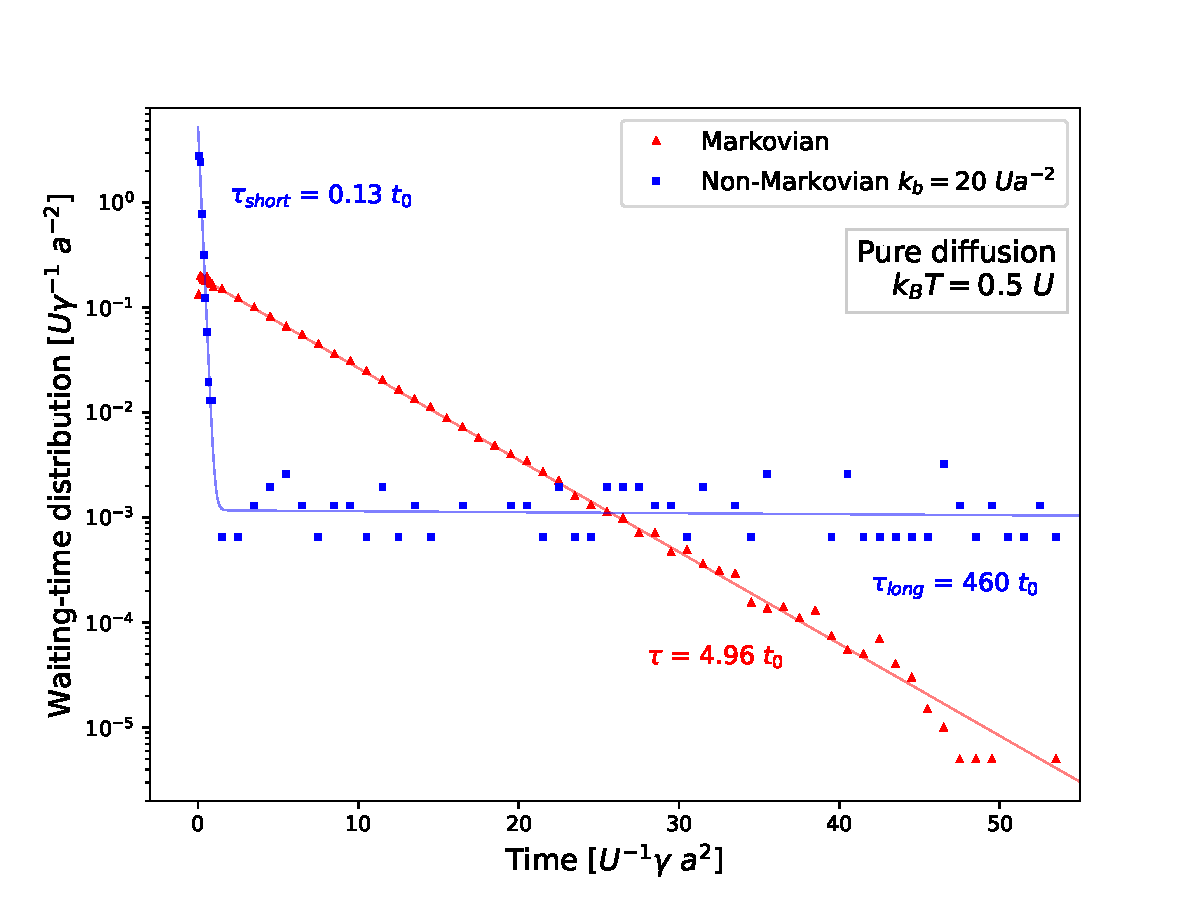
\includegraphics[width=\textwidth]{kb20_T05.pdf}
    \caption{Same as Figure \ref{P_kb15}, but for a viscoelastic spring $k_b=20\hspace{0.1cm}Ua^{-2}$}
    \label{P_kb20}
\end{figure}
Note that in Figure \ref{P_kb20} the histograms have a different bin width compared to those in Figure \ref{P_kb15}, more precisely, a bin width of $2\hspace{0.1cm}t_0$ is set from $1\hspace{0.1cm}t_0$ onwards. This is because, with a higher coupling constant $k_b$, the number of barrier crossing events is lower, requiring the merging of more times to obtain useful statistics.
\clearpage
\subsection{Temperature effect on Brownian motion}
Here we investigate how temperature influences the waiting-time distributions $P(t_\text{w})$. In particular, to study this effect, we compare the waiting-time distributions of a simple Brownian particle and a Brownian particle with memory when $k_BT=0.7\; U$.
\begin{figure}[ht!]
    \centering
    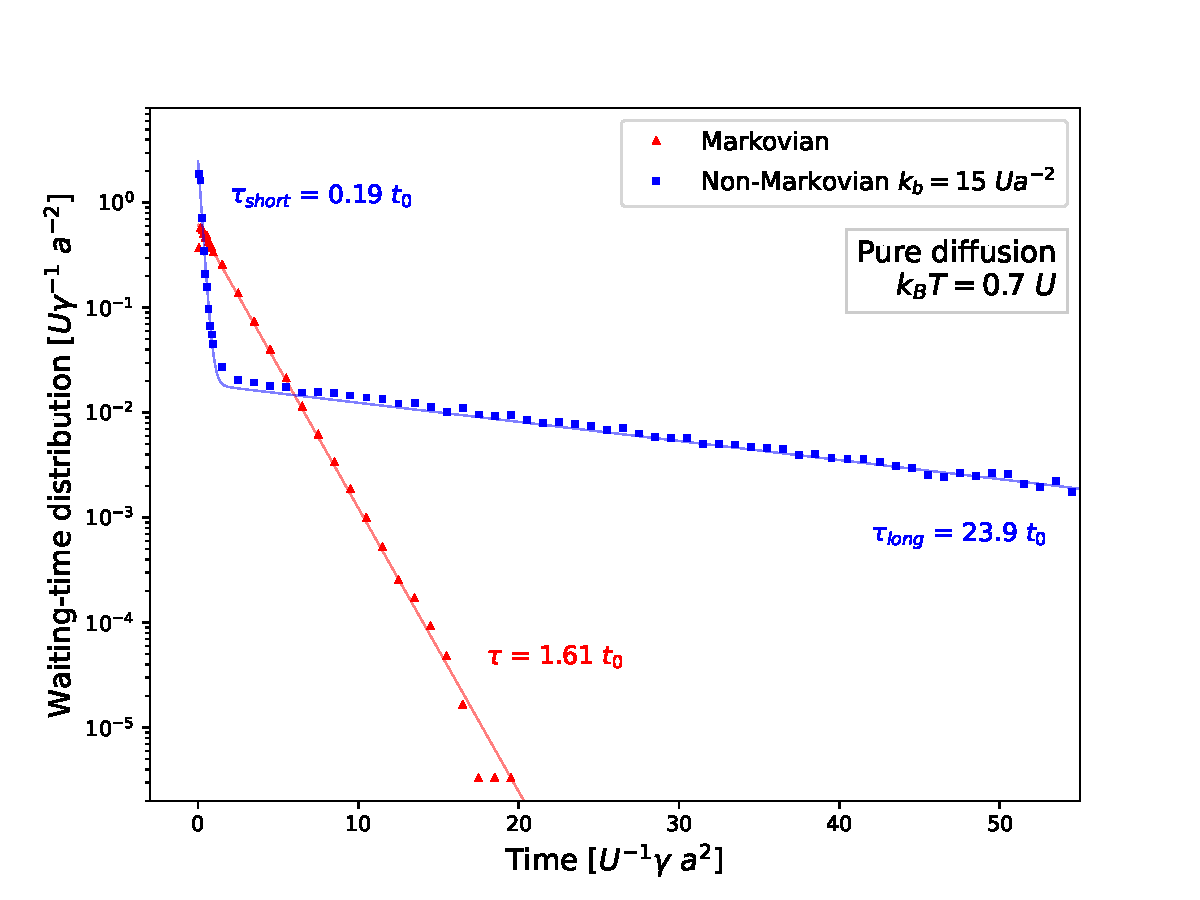
\includegraphics[width=0.9\textwidth]{kb15_T07.pdf}
    \caption{Same as Fig.~\ref{P_kb15}, but for $k_BT = 0.7\hspace{0.1cm}U$}
    \label{fig:kb15_temp_high}
\end{figure}
In both scenarios the decays exhibit shorter characteristic times $\tau$ compared to lower temperature $k_BT=0.5\; U$. $\tau_\text{long}$ is significantly affected, while $\tau_\text{short}$ remains nearly the same, as it is mainly affected by the viscoelastic spirng $k_b$. This effect is due to the presence of larger stochastic forces, causing the particle to exit the potential minima more rapidly.
\begin{table}
\centering 
\begin{tabular}{ccc}
    \toprule
    Fit parameter & $k_BT = 0.5\hspace{0.1cm}U$ & $k_BT = 0.7\hspace{0.1cm}U$ \\
    \midrule
    $\tau_\text{short} \hspace{0.1cm} [t_0]$ & $0.171\pm 0.009$ & $0.19 \pm 0.01$\\[0.5ex]
    $\tau_\text{long} \hspace{0.25cm} [t_0]$ & $221 \pm 12$ & $23.9 \pm 0.3$\\[0.5ex]
    
    
    \bottomrule
\end{tabular}
\caption{Comparison of characteristic times of Brownian diffusion with memory $k_b=15\hspace{0.1cm}Ua^{-2}$ of two different temperatures}
\label{tab:variando_kbt}
\end{table}
\clearpage
\subsection{Standard Prandtl-Tomlinson model}
\label{sec:spiegobinning}
We come now to investigate the distribution of waiting times $P(t_\text{w})$ for the standard Prandtl-Tomlinson model, i.e. without considering a viscoelastic environment($k_b=0$), but including driving through a spring with $K=10^{-3}\hspace{0.1cm}Ua^{-2}$. In these simulations $k_BT$ is set to $0.5\hspace{0.1cm}U$.
\begin{figure}
    \centering
    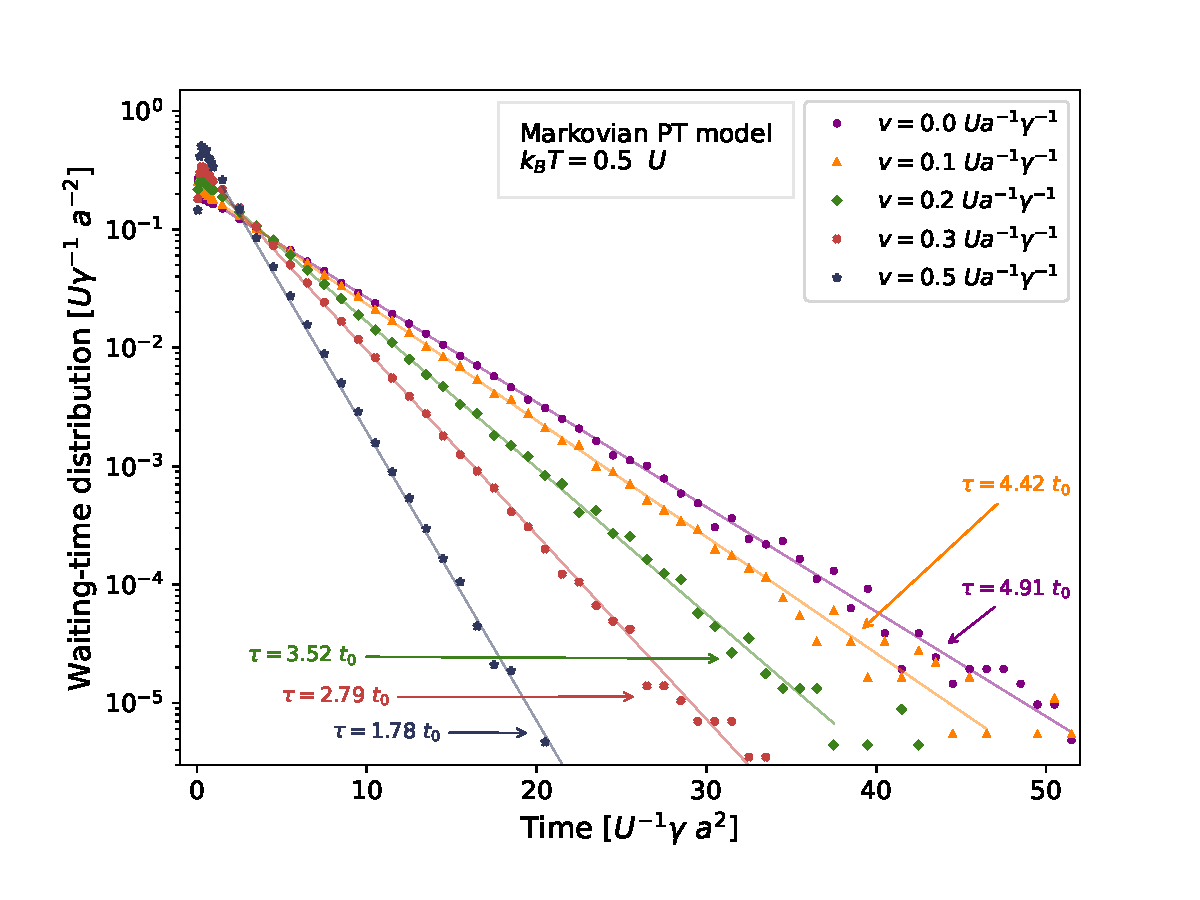
\includegraphics[width=\textwidth]{standard_PT_definitivo.pdf}
    \caption{Waiting times distribution $P(t_\text{w})$ of a standard PT model ($k_b=0$) for a few values of the the sliding velocity $v$ and fixed parameters $K=0.001\, Ua^{-2}$ and $k_BT=0.5\hspace{0.1cm}U$.}
    \label{fig:simplePT}
\end{figure}
\\
Figure \ref{fig:simplePT} reports a few histograms of the standard PT model driven at few different velocities. The $v=0$ simulation yields the distribution of waiting times of a simple Brownian particle constrained with a spring of elastic constant $K$ to a fixed point: this is similar to the free model, and we take it as the reference to compare the $v>0$ simulations. The waiting-time distributions exhibit long timescale exponential decays with decreasing characteristic time values $\tau$ as a function of $v$. This is expected since a larger slider velocity reduces the probability of longer waiting times favoring shorter stays in the potential minima.
\begin{table}
\centering 
\begin{tabular}{cc}
    \toprule
    Velocity $v$ [$U \gamma ^{-1} a^{-1}$] & Fit parameter $\tau$ [$t_0$]  \\
    \midrule 
    $0.0$ & $4.91\pm 0.04$\\
    $0.1$ & $4.42 \pm 0.04$ \\
    $0.2$ & $3.52\pm 0.02$\\
    $0.3$ & $2.79\pm 0.02$ \\
    $0.5$ & $1.78 \pm 0.03$ \\
    \bottomrule
\end{tabular}
\caption{Parameters of waiting times distribution $P(t_\text{w})$ for standard Prandtl-Tomlinson model}
\label{tab:simplePT}
\end{table}
Table \ref{tab:simplePT} reports the characteristic times $\tau$ obtained through a linear fit over the natural logarithms of bin heights, performed using the appropriate NumPy function. The fitting is performed from the first bin after the peak in the distribution to the one before the first empty bin, beyond which data become unreliable. This protocol of bin range for fitting single exponential decays is also applied to all subsequent fits.

\subsection{Non-Markovian Prandtl-Tomlinson model}
In this section we aim to understand how the distributions of waiting times in potential minima change when considering our non-Markovian Prandtl-Tomlinson model compared to the regular PT model under analogous driving conditions.
\begin{figure}
    \centering
    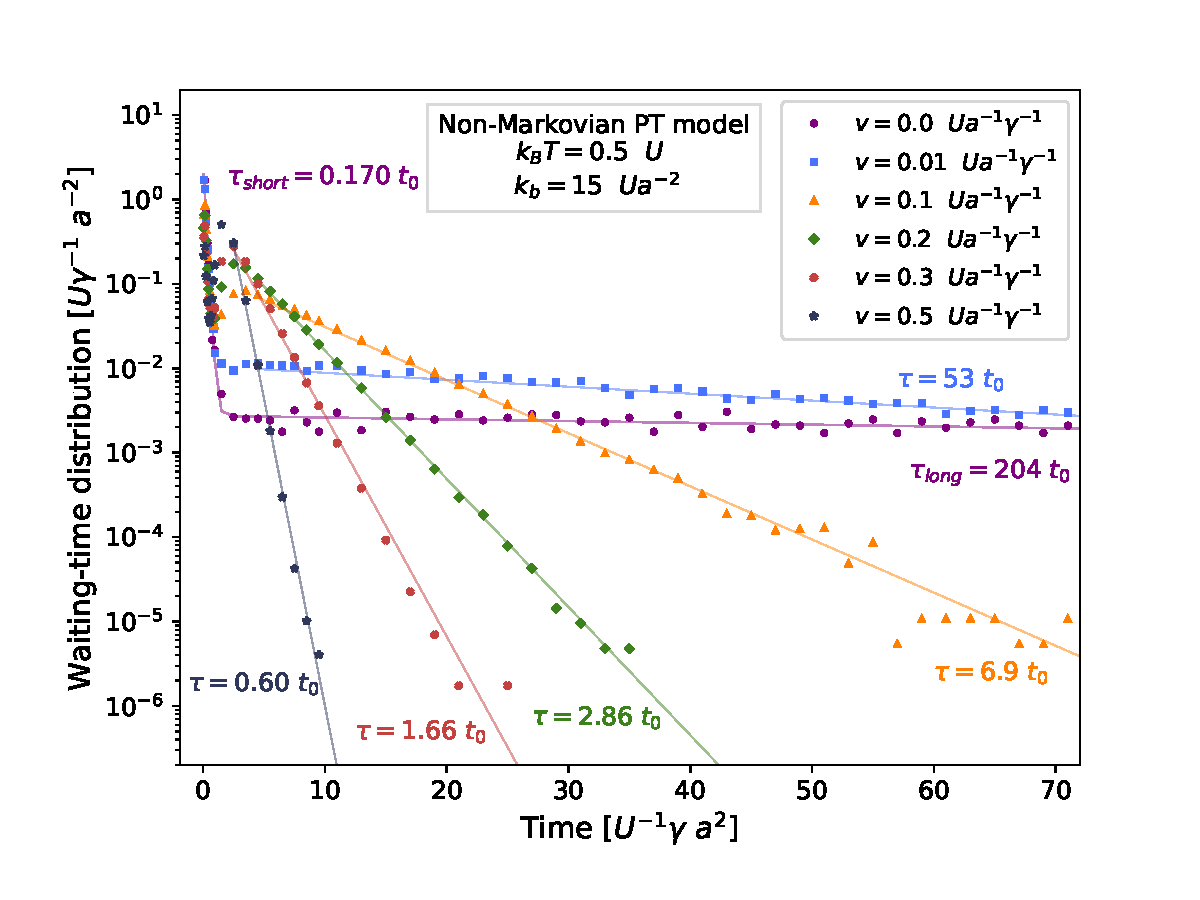
\includegraphics[width=0.9\textwidth]{istogramma_confronto_kb15_def.pdf}
    \caption{Same as Fig.~\ref{fig:simplePT} but for the non-Markovian thermostat, characterized by $k_b=15\hspace{0.1cm}Ua^{-2}$}
    \label{fig:confronto_velocità_kb15}
\end{figure}
Figure \ref{fig:confronto_velocità_kb15} reports six distributions of waiting times as a function of the slider velocity, from $0$ to $0.5 \hspace{0.1cm} U a^{-1} \gamma^{-1}$, while fixing the coupling parameters $k_b=15\hspace{0.1cm}Ua^{-2}$. The figure also reports the values of large-$t_\text{w}$ decay times $\tau$ for each distribution. These values are obtained following the same protocol described in Subsection \ref{sec:spiegobinning}. Like for the Markovian model, increasing the slider velocity results in fewer occurrences of longer waiting times. It may also be observed that, as $v$ increases, the waiting time distributions, after a rapid exponential decay at short timescales, related to the viscoelastic rapid back-and-forth events, exhibit an non monotonic trend characterised by a peak followed by the typical exponential decay at longer timescales. This peak becomes more pronounced and shifts to lower $t_\text{w}$ as the dragging velocity increases, as can be seen in the detail of the waiting-time distributions reported in Figure \ref{fig:zoom_kb15}.
\begin{figure}
    \centering
    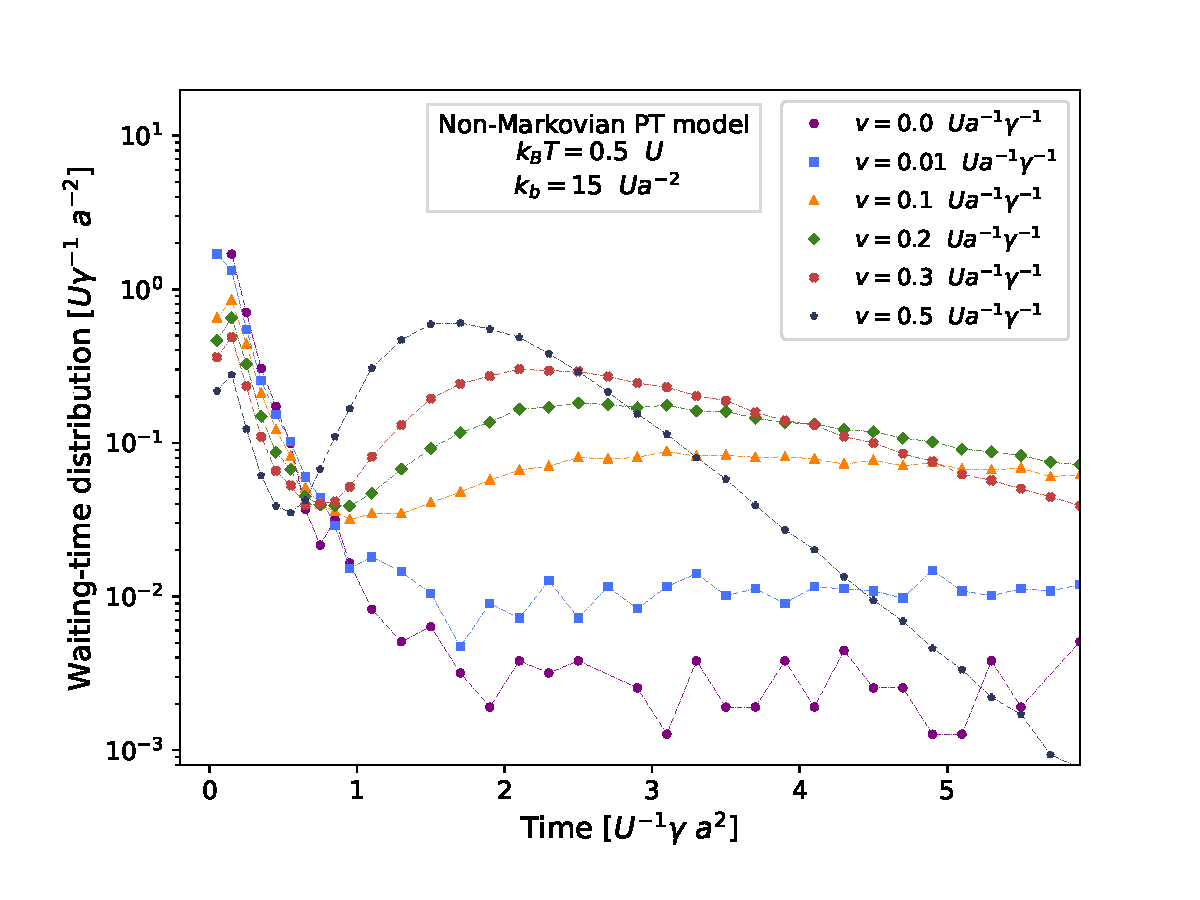
\includegraphics[width=0.9\textwidth]{zoom_kb15.pdf}
    \caption{Detail of Fig. \ref{fig:confronto_velocità_kb15} using a bin width of $0.1\hspace{0.1cm}t_0$, from $0$ to $t_0$, and $0.2\hspace{0.1cm}t_0$ onward}
    \label{fig:zoom_kb15}
\end{figure}
\newpage
In particular, the formation of this peak is due to the presence of a characteristic waiting time $t_\text{ave}$ in a minimum, namely the average time between two consecutive minima at the dragging velocity $v$
\begin{equation}
    t_\text{ave} = \dfrac{a}{v}\, ,
\end{equation}
namely the inverse of the washboard frequency of the PT model.

Figure \ref{fig:confronto_velocità_kb20} shows the same comparison as Figure \ref{fig:confronto_velocità_kb15} using a different value of the viscoelastic coupling spring $k_b=20\hspace{0.1cm}Ua^{-2}$.
\begin{figure}
    \centering
    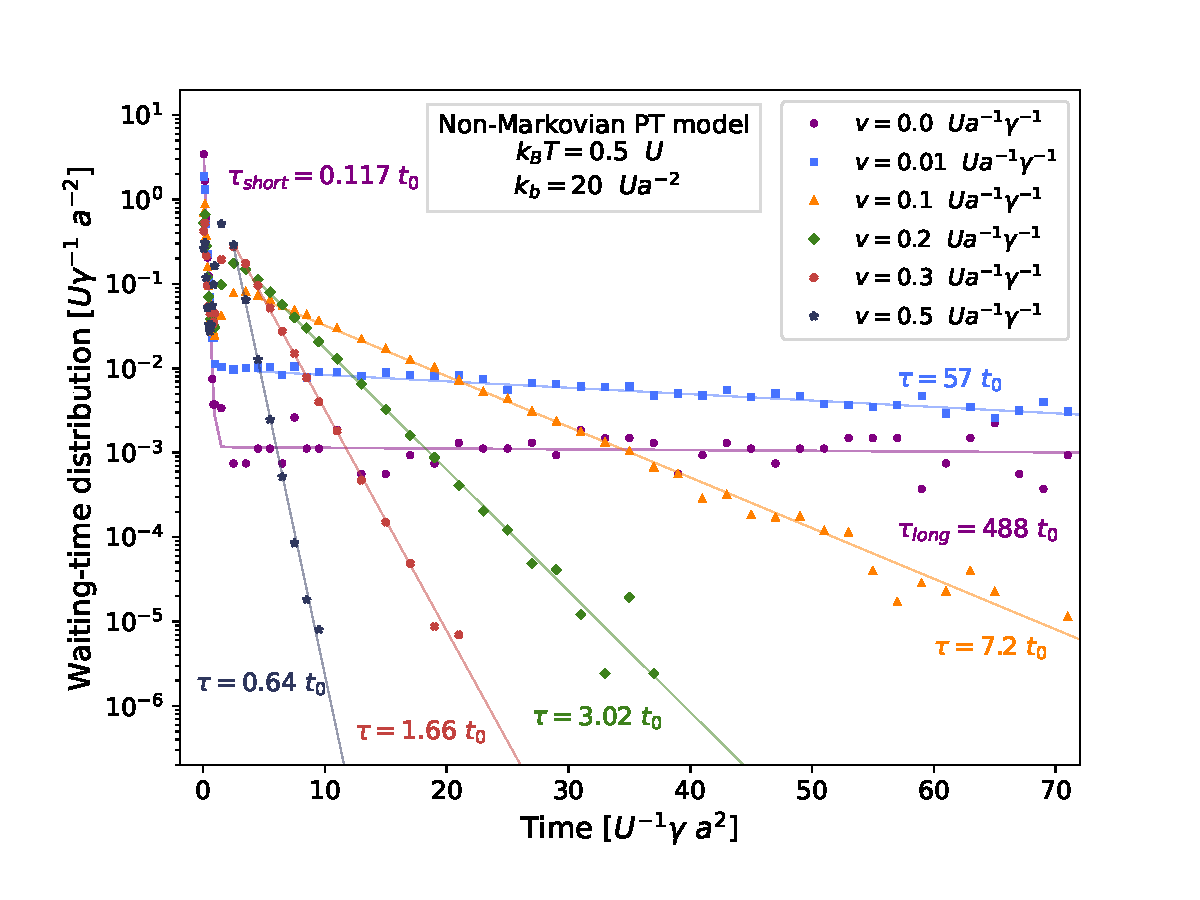
\includegraphics[width=\textwidth]{istogramma_confronto_kb20_def.pdf}
    \caption{Same as Fig.~\ref{fig:confronto_velocità_kb15}, but for $k_b=20\hspace{0.1cm}Ua^{-2}$.}
    \label{fig:confronto_velocità_kb20}
\end{figure}
The effect of a stronger coupling with the viscoelastic bath is to keep the particle for longer times in the potential minima, consistent with higher effective barriers see Fig.~\ref{fig:effpotenz}. Comparing $k_b=15\hspace{0.1cm}Ua^{-2}$ and $k_b=20\hspace{0.1cm}Ua^{-2}$, the characteristic times $\tau$ undergo minor changes, see also Table \ref{tab:tau}.
\begin{table}
\centering 
\begin{tabular}{ccc}
    \toprule
    Velocity [$U \gamma ^{-1} a^{-1}$] & \multicolumn{2}{c}{Fit parameter $\tau$  [$t_0$]} \\
    \cmidrule(lr){2-3}
    & $k_b = 15$  [$Ua^{-2}$]& $k_b = 20$  [$Ua^{-2}$] \\
    \midrule 
    $0.01$ & $52.8\pm 0.9$ & $57 \pm 1$\\
    $0.1$ & $6.9 \pm 0.2$ & $7.2 \pm 0.1$\\
    $0.2$ & $2.86\pm 0.04$ &$3.02 \pm 0.09$\\
    $0.3$ & $1.66\pm 0.06$  &$1.66 \pm 0.02$\\
    $0.5$ & $0.60 \pm 0.02$  &$0.64 \pm 0.02$\\
    \bottomrule
\end{tabular}
\caption{Large-$t_\text{w}$ decay time of the distribution $P(t_\text{w})$ for the non-Markovian Prandtl-Tomlinson model and two different viscoelastic couplings $k_b$.}
\label{tab:tau}
\end{table}
\begin{figure}
    \centering
    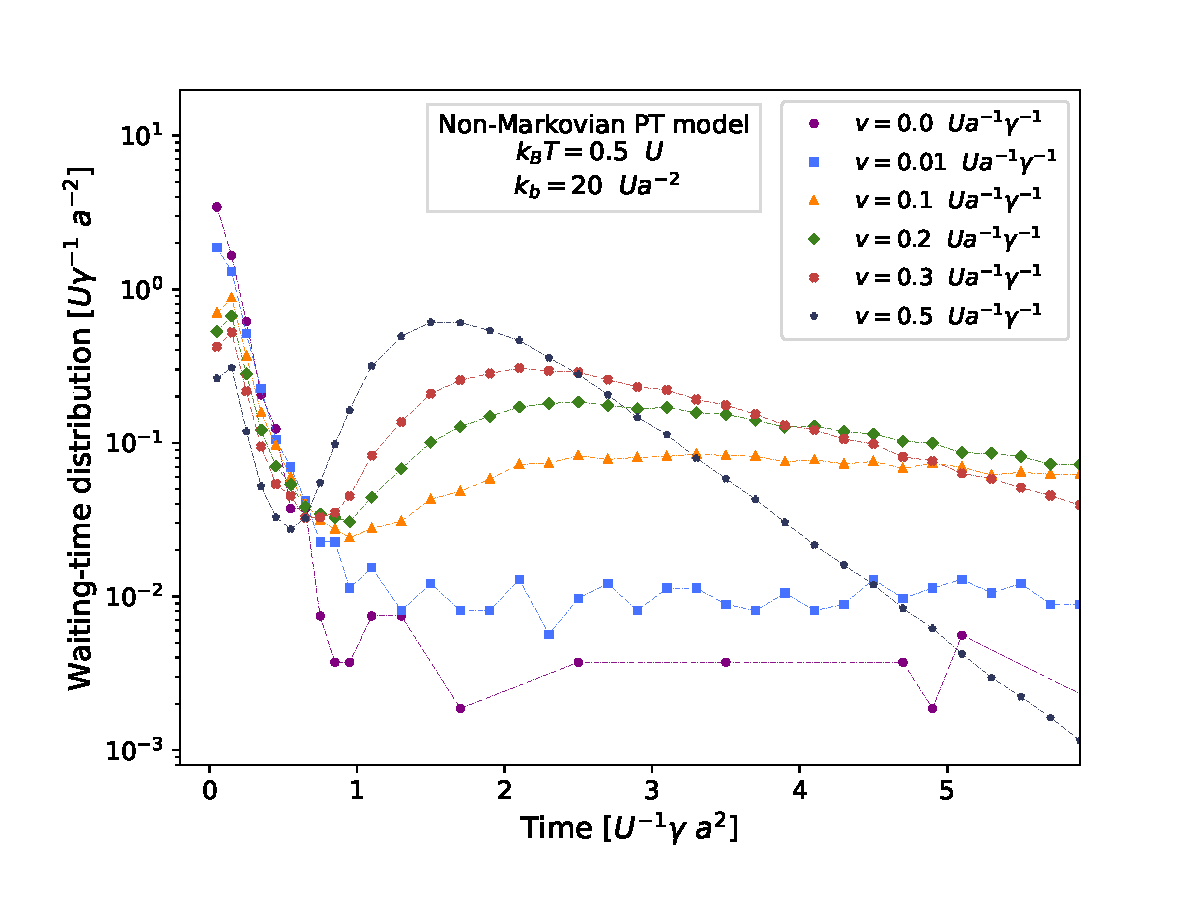
\includegraphics[width=\textwidth]{zoom_kb20.pdf}
    \caption{Same as Fig.~\ref{fig:zoom_kb15}, but for $k_b=20\, Ua^{-2}$.}
    \label{fig:zoom_kb20}
\end{figure}
\clearpage
\subsection{Left and right barrier crossings}
It is instructive to separately examine the distributions of crossings made to the left (backward) and to the right (forward). We define the right crossing waiting time as the waiting time in a minimum before a forward crossing occurs, namely a displacement of at least $0.7\hspace{0.1cm}a$ forward. The left crossing waiting time is defined similarly.

In particular, it is interesting to analyze left and right crossings waiting times by varying the velocity from $0$ to $0.5 \hspace{0.1cm} U a^{-1} \gamma^{-1}$. As expected, for zero velocity the distributions are practically identical, which is consistent with the fact that, under 'no-sliding' conditions, there is no preferred direction for barrier crossings, and they are evenly distributed in both directions due to thermal fluctuations.
\begin{figure}[ht!]
    \centering
    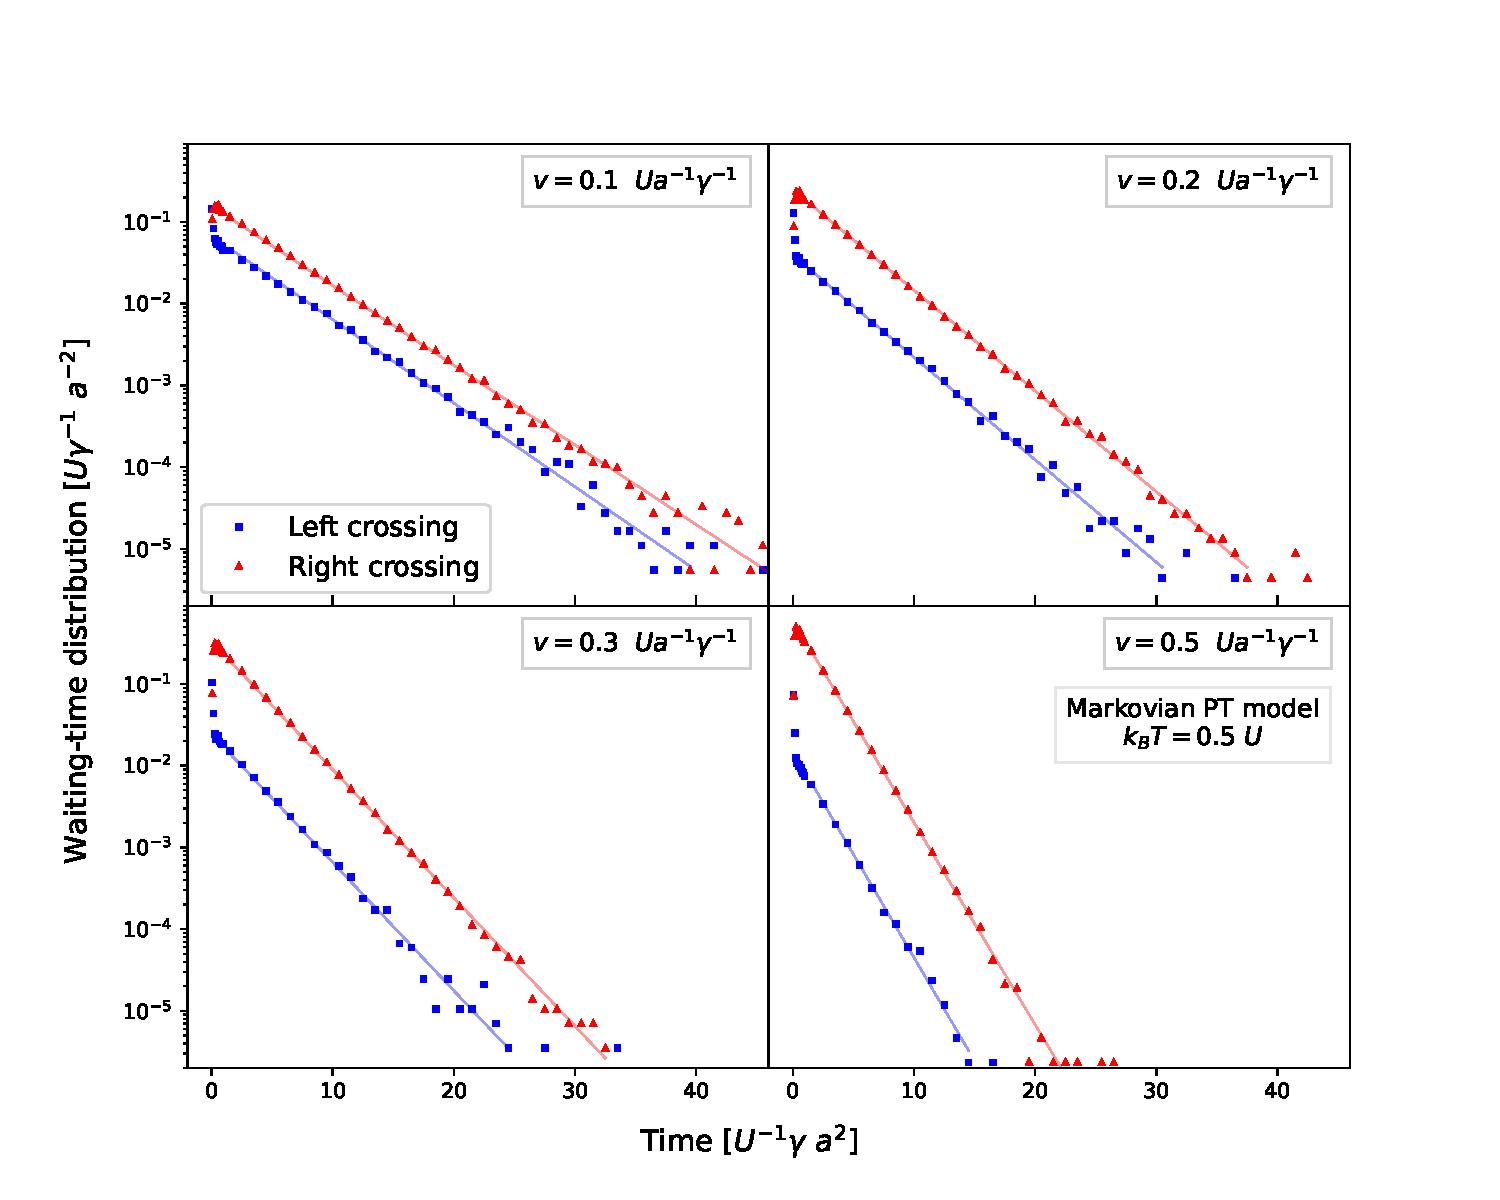
\includegraphics[width=\textwidth]{sxdx_simplePT_DEFINITIVO.pdf}
    \caption{Leftward (squares) and rightward (triangles) barrier crossings waiting-time distributions $P(t_\text{w})$ for the standard Markovian Prandtl-Tomlinson model for a few values of driving velocity $v$}
    \label{fig:simplePT_sxdx}
\end{figure}

The standard Prandtl-Tomlinson model exhibits decreasing similar characteristics times, but different ratios of barrier-crossing events as $v$ is increased, thus a different value of the prefactor. In both distributions the longer waiting times are suppressed as $v$ is increased, see Table \ref{tab:sxdx_simplePT}.
\begin{table}
\centering 
\begin{tabular}{ccc}
    \toprule
    Velocity [$U \gamma ^{-1} a^{-1}$] & Leftward $\tau_\text{left} $[$t_0$] & Rightward $\tau_\text{right} $[$t_0$]\\
    \midrule 
    $0.1$ & $4.24 \pm 0.07$ & $4.46 \pm 0.08$\\
    $0.2$ & $3.47 \pm 0.06$ & $3.52 \pm 0.02$ \\
    $0.3$ & $2.77 \pm 0.09$ & $2.77 \pm 0.03$\\
    $0.5$ & $1.71\pm 0.04$ & $1.77 \pm 0.04$\\
    \bottomrule
\end{tabular}
\caption{Characteristic times for the leftward and rightward-jumps waiting-time distribution $P(t_\text{w})$ for the Markovian Prandtl-Tomlinson model.}
\label{tab:sxdx_simplePT}
\end{table}

\begin{figure}
\centering
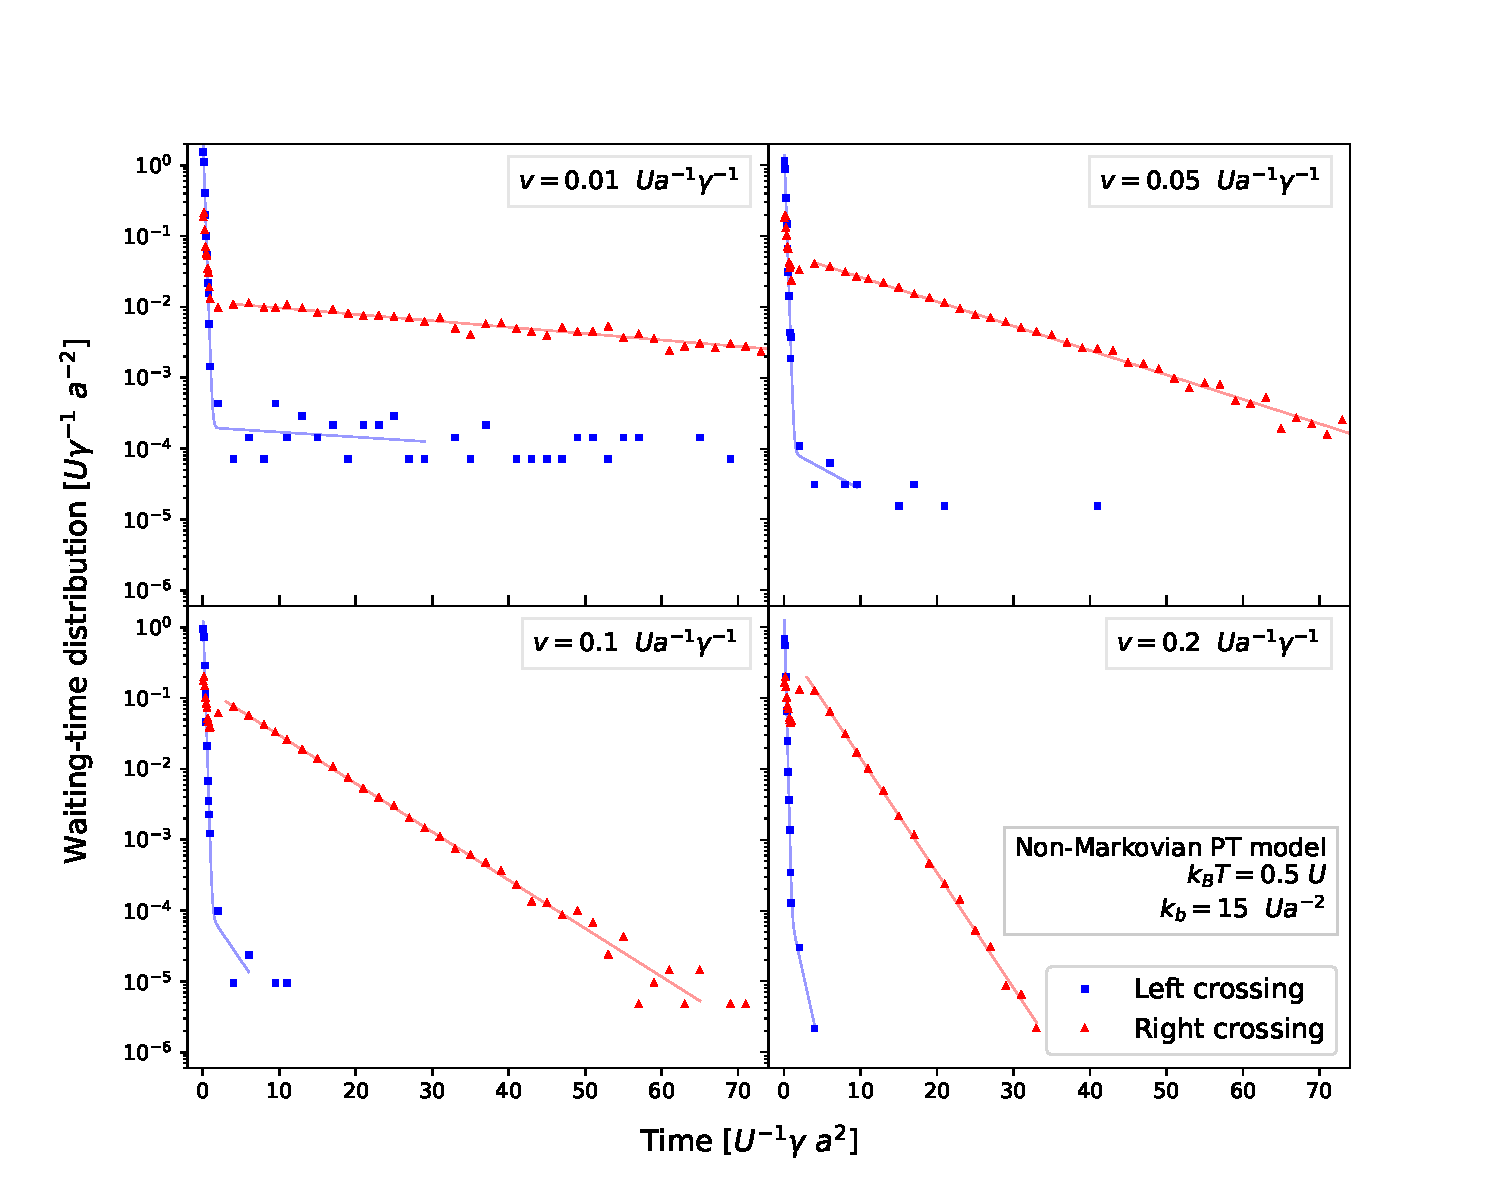
\includegraphics[width=\textwidth]{isto_sxdx_kb15_basseV.pdf}
\caption{Same as Fig. \ref{fig:simplePT_sxdx} but for the non-Markovian Prandtl-Tomlinson model with $k_b=15\; Ua^{-2}$.}
\label{fig:sxdx_kb15_basseV}
\end{figure}
The non-Markovian PT model instead develops a radical asymmetry in the left versus right distributions, even at moderate speed. Specifically, we notice two very different behaviors when considering the waiting time preceding a right barrier crossing compared to that of a left crossing. When the crossing is performed to the right, the characteristic time decreases as the velocity of the slider increases. However, for the left crossing, the characteristic time remains relatively similar and much shorter than that of the rightward jumps. For the rightward distributions we execute a linear fit over the logarithm of the right-crossing waiting-time distribution, which shows a single exponential decay on the long timescale. In contrast we fit the left crossing waiting-time distribution with a short timescale a sum of two exponentials. To evaluate whether the left crossing waiting times distribution exhibits a double exponential decay,
we computed the waiting-time distribution from $v=0.01\; Ua^{-1}\gamma^{-1}$ to $v=0.5\; Ua^{-1}\gamma^{-1}$.

Note that the histograms in Figure \ref{fig:simplePT_sxdx} have a bin width of $0.1 t_0$ from $0$ to $ t_0$, and then $t_0$ onwards. Instead, the histograms in Figures \ref{fig:sxdx_kb15_alteV} and \ref{fig:sxdx_kb15_basseV} have the same bin width, as Figure \ref{fig:simplePT_sxdx}, in the initial region, but in the $t_\text{w}>t_0$ region, they have different widths. For the histograms of waiting times before a rightward crossing, the bin width is set to $1 t_0$, while for the leftward waiting times, we adopt a bin width of $2 t_0$ to collect more of these rarer events, resulting in a sufficient number of data points for a fair statistics.
\begin{figure}
    \centering
    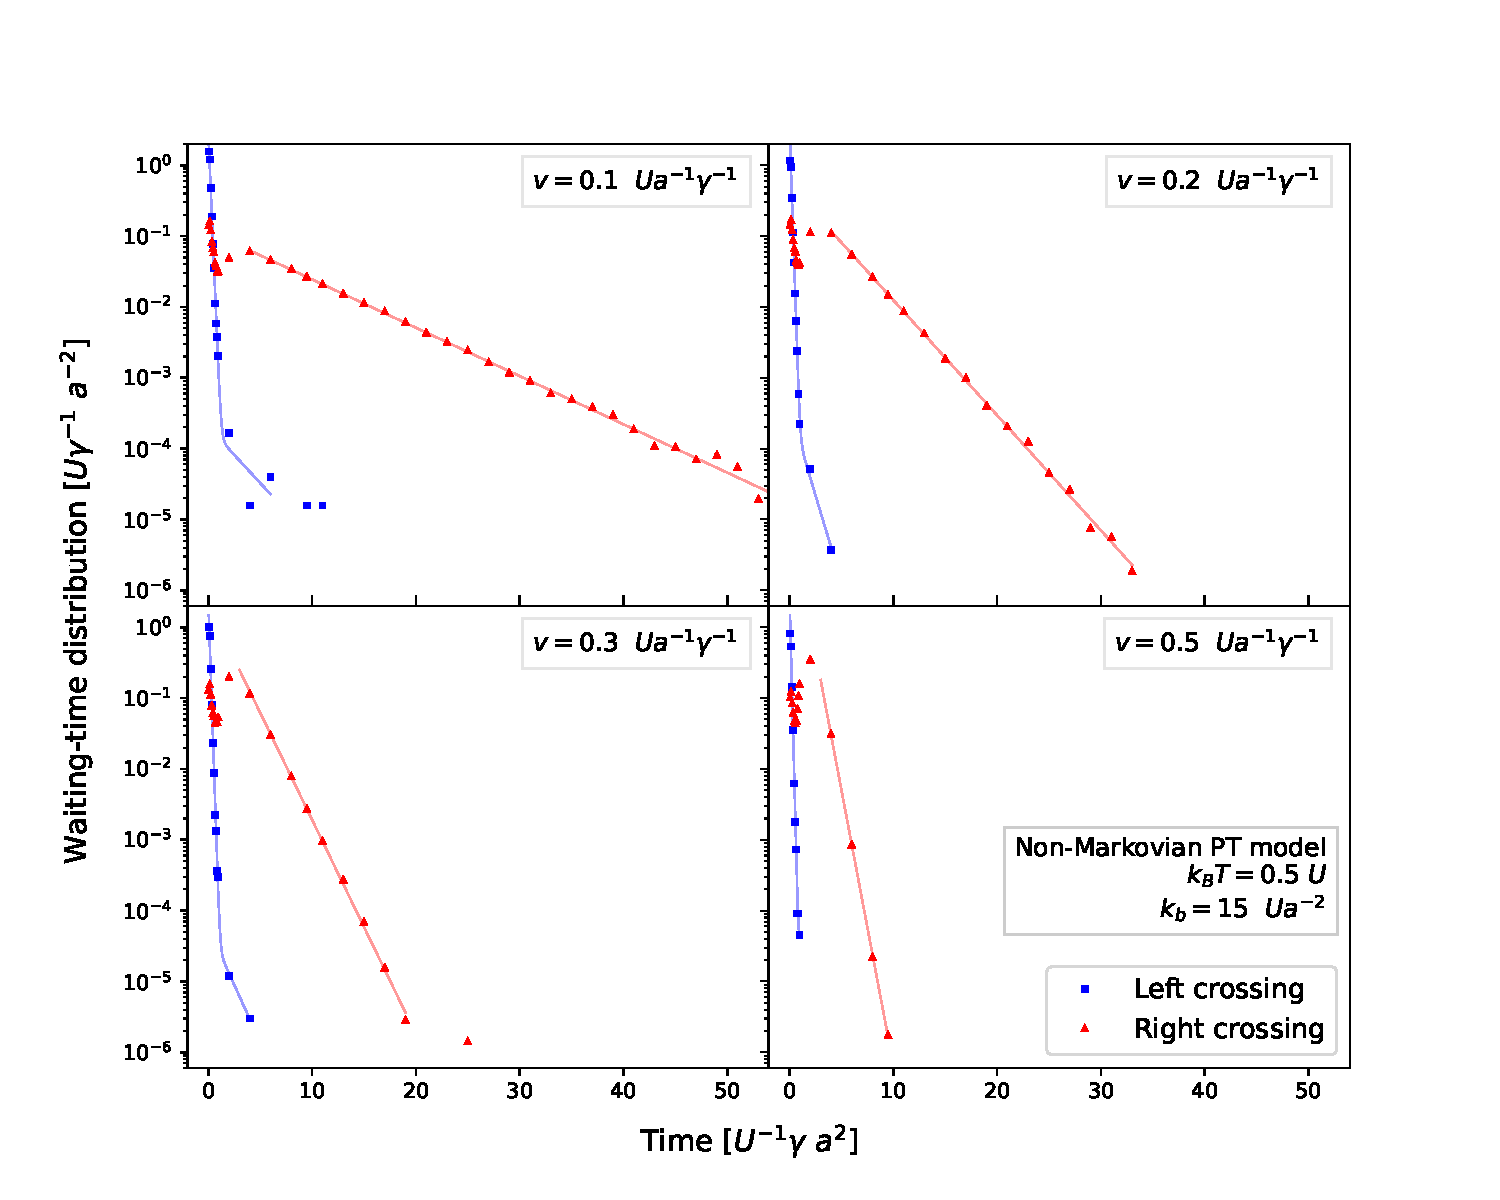
\includegraphics[width=\textwidth]{isto_sxdx_kb15_alteV.pdf}
    \caption{Same as Fig. \ref{fig:sxdx_kb15_basseV} but for higher velocities.}
    \label{fig:sxdx_kb15_alteV}
\end{figure}
\newpage
\noindent In Figure \ref{fig:sxdx_kb15_basseV}, we observe the double exponential decay of the waiting times distribution more clearly at lower speeds. Additionally, at slow driving the particle can remain for tens of time units before performing a leftward barrier crossing. Table \ref{tab:sxdx_right} reports the obtained characteristic times for the exponential decays of the rightward crossing waiting-time distribution
\begin{table}
\centering 
\begin{tabular}{ccc}
    \toprule
    Velocity [$U \gamma ^{-1} a^{-1}$] & Fit parameter $\tau $[$t_0$] \\
    \midrule 
    $0.01$ & $47.9 \pm 0.9$\\
    $0.05$ & $12.6 \pm 0.3$\\
    $0.1$ & $6.4 \pm 0.1$ \\
    $0.2$ & $2.67 \pm 0.03$ \\
    $0.3$ & $1.44 \pm 0.02$ \\
    $0.5$ & $0.560 \pm 0.006$ \\
    \bottomrule
\end{tabular}
\caption{Characteristic times for the rightward-jumps waiting-time distribution $P(t_w)$ for non-Markovian Prandtl-Tomlinson model with $k_b=15\; Ua^{-2}$}
\label{tab:sxdx_right}
\end{table}
\\Table \ref{tab:sxdx_left} reports the characteristic times for the two-exponential decays of the leftward crossing waiting times distribution
\begin{table}
\centering 
\begin{tabular}{ccc}
    \toprule
    Velocity [$U \gamma ^{-1} a^{-1}$] & Fit parameter $\tau_{short} [t_0]$ & Fit parameter $\tau_{long} [t_0]$ \\
    \midrule 
    $0.01$ & $0.13 \pm 0.01$ & $63 \pm 17$\\
    $0.05$ & $0.132\pm 0.008$ & $7 \pm 4$\\
    $0.1$ & $0.124 \pm 0.009$ & $3\pm 1$\\
    $0.2$ & $0.099 \pm 0.005$ & $-$\\
    $0.3$ & $0.097 \pm 0.004$ & $-$\\
    $0.5$ & $0.076 \pm 0.005$ & $-$\\
    \bottomrule
\end{tabular}
\caption{Characteristic times for the leftward-jumps waiting-time distribution $P(t_w)$ for non-Markovian Prandtl-Tomlinson model with $k_b=15\; Ua^{-2}$}
\label{tab:sxdx_left}
\end{table}
\\
As can be inferred from Figure \ref{fig:sxdx_kb15_alteV} when the slider velocity exceeds $0.2 \hspace{0.1cm} U\gamma^{1} a^{-1}$ the estimated characteristic time for exponential decay on long timescales has no significance due to the scarcity of points.

\clearpage
\section{Velocity dependence of friction}
In this section we investigate the friction force in the Markovian Prandtl-Tomlinson model and its non-Markovian extension. Specifically, we address the driving-velocity dependence. Section \ref{PTmodel} illustrates the relation between the velocity of the slider and the friction force of the standard PT model. In particular, in the high velocity regime the time-averaged friction force is expected to a linear dependence on slider velocity, while in a low velocity regime the friction force is expected to exhibit a logarithmic dependence on slider velocity, see Eq.\eqref{eq:friction}.
\begin{figure}
    \centering
    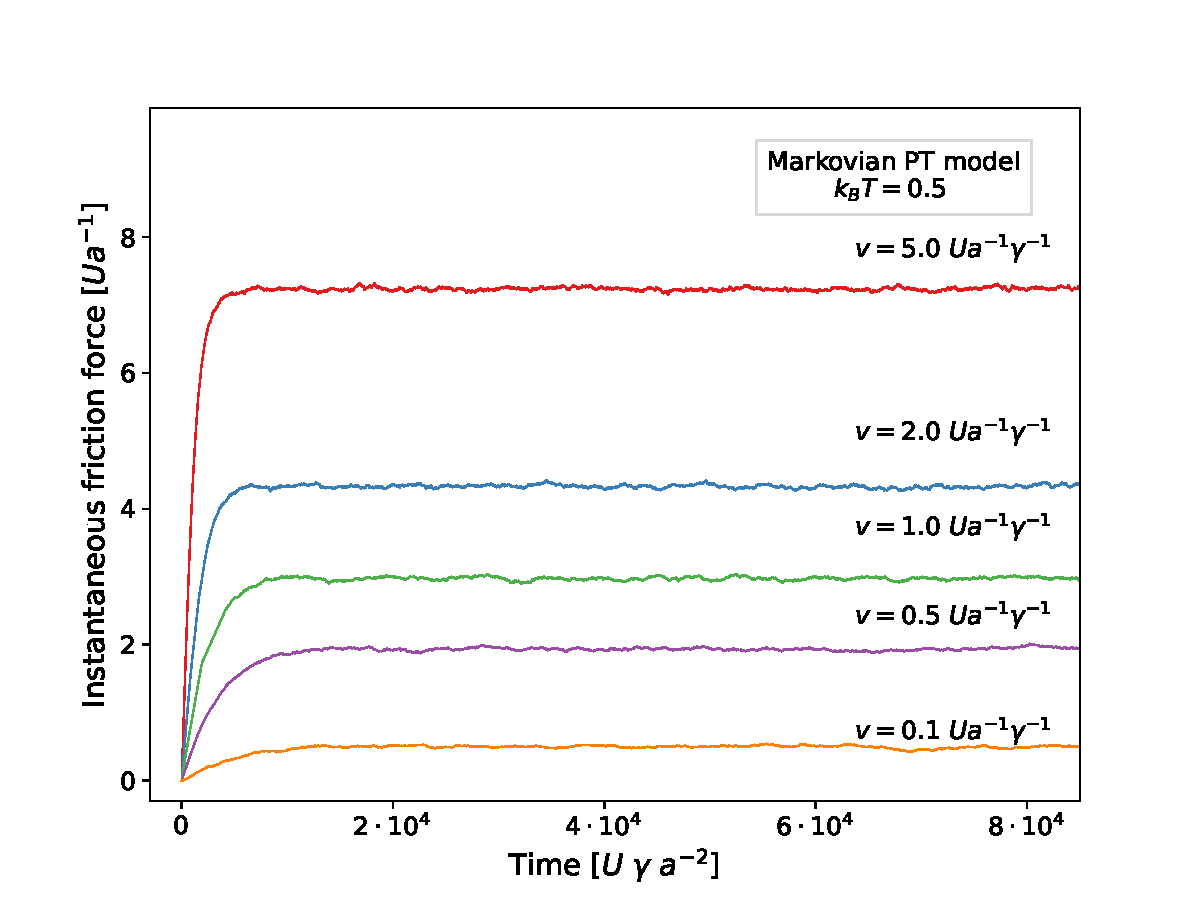
\includegraphics[width=\textwidth]{alteV_kb0_forzaplot.pdf}
    \caption{Instantaneous friction force for a few driving velocities $v$ in the standard Markovian PT model.}
    \label{fig:friction_kb0_high_velocities}
\end{figure}
In the Prandtl-Tomlinson model, the friction force can be evaluated from the elastic force associated with the elongation of the spring coupling the slider to the colloidal particle. This elastic force is described by the equation
\begin{equation}
    F_k(v,t) = K\Delta x = K (x_\text{slider} - x) = K(vt -  x)\; .
\end{equation}
Here the slider position $x_\text{slider}$ is simply given by the product of its constant velocity and time.

Figure \ref{fig:friction_kb0_high_velocities} compares the time dependence of the instantaneous friction forces in the standard Prantl-Tomlinson model, using $K=0.001\;Ua^{-2}$, amplitude $2U$ and lattice spacing $a$, for a few values of velocity, from $v=0.1\hspace{0.1cm}U\gamma^{-1} a^{-1}$ to $v=5\hspace{0.1cm}U\gamma^{-1} a^{-1}$. 
\begin{figure}[ht!]
    \centering
    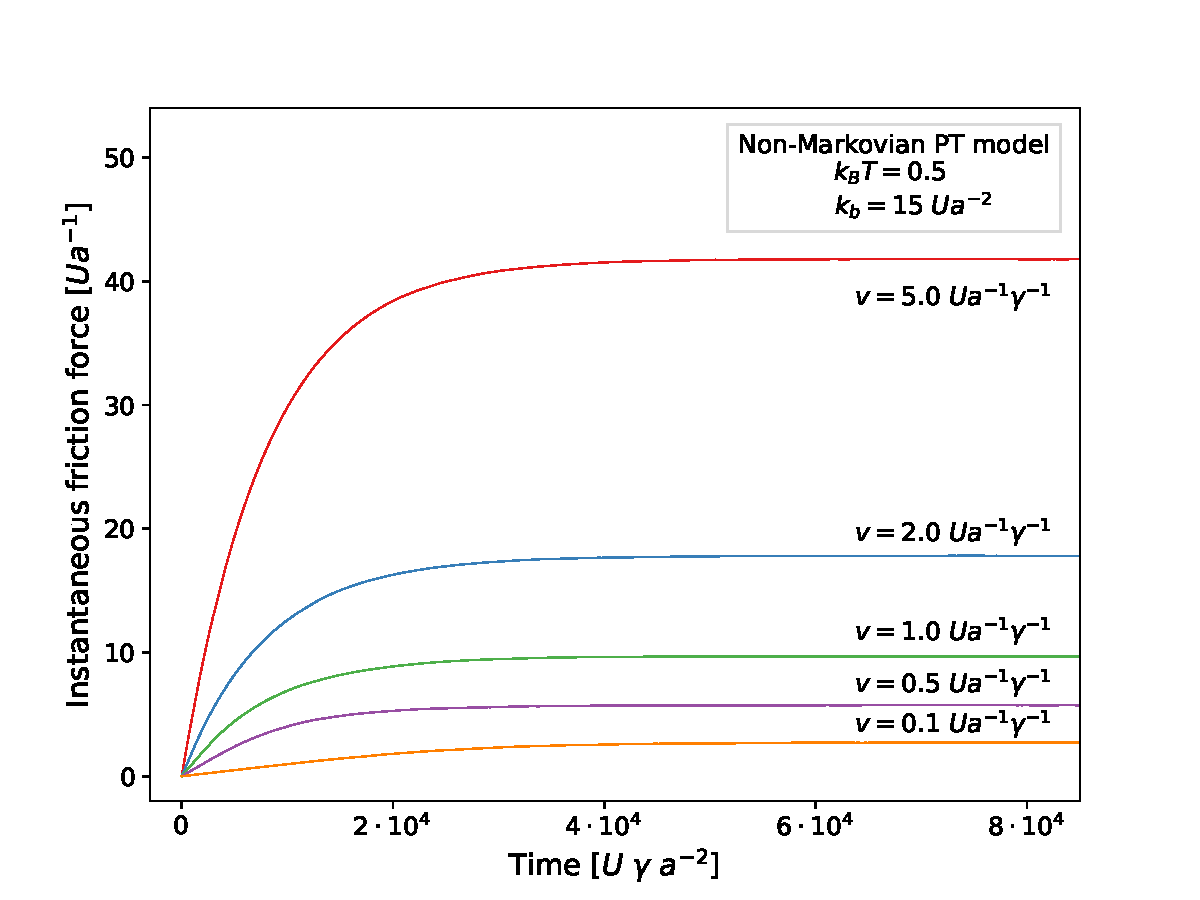
\includegraphics[width=\textwidth]{alteV_kb15_forzaplot.pdf}
    \caption{Instantaneous friction force for a few driving velocities $v$ in the non-Markovian PT model with $k_b=15\; Ua^{-2}$.}
    \label{fig:friction_kb15_high_velocities}
\end{figure}

Similarly, Figure \ref{fig:friction_kb15_high_velocities} compares the friction forces in the non-Markovian PT model as a function of time for the same driving velocities, and for $k_b=15\hspace{0.1cm}Ua^{-2}$.
In both these two figures, it is evident that initially the particle lags many length units behind the tracer.

This initial transient needs to be omitted in the evaluation of the time-averaged friction: we compute the average force starting after the end of the transient, when the force stabilizes. As recalled above, in this regime, for the standard overdamped PT model, the dependence of the friction force on velocity is linear, as verified in Figure \ref{fig:high_velo_friction}. The non-Markovian PT model too exhibits a linear dependence on velocity, but with a much larger slope,the result of the coupling with an environment characterized by a higher dissipation coefficient $\gamma_b$ compared to that of the particle $\gamma$.
\begin{figure}
    \centering
    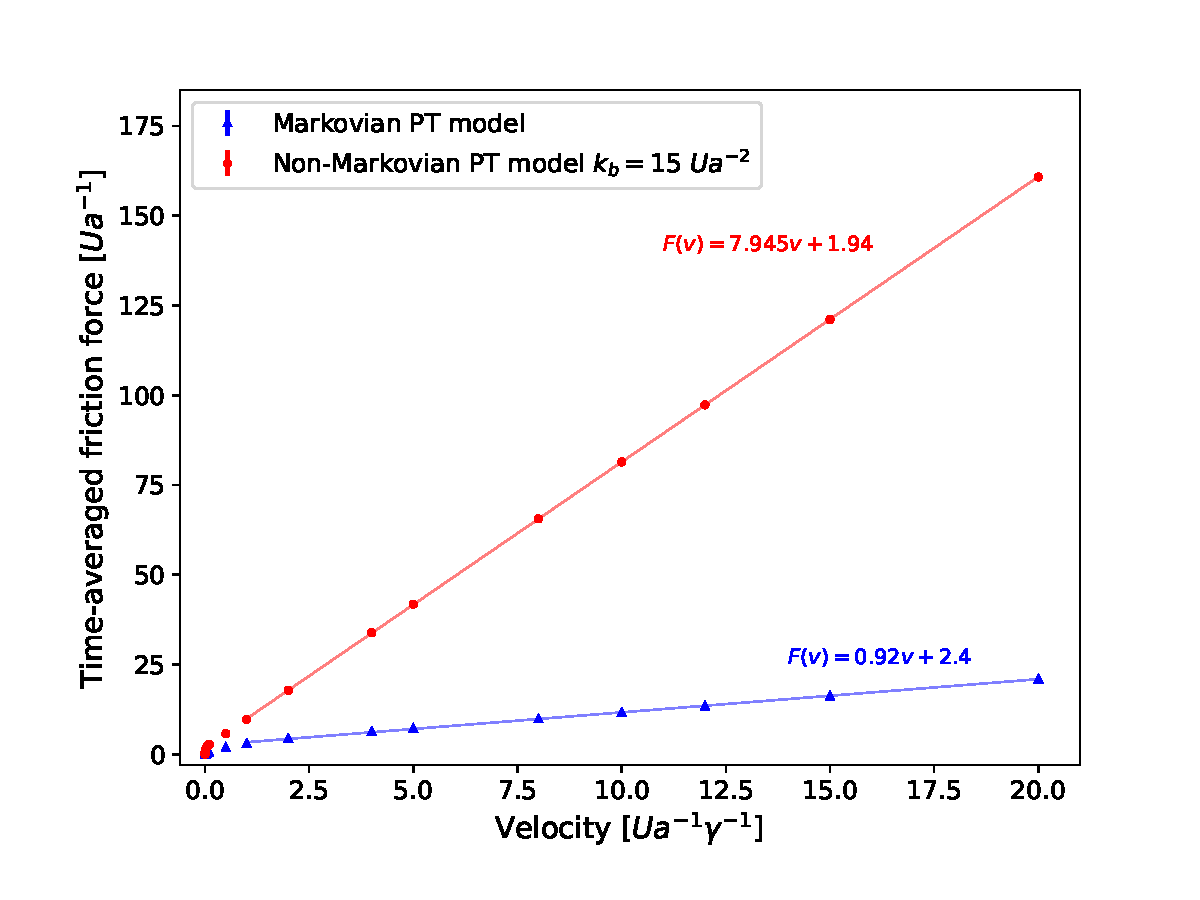
\includegraphics[width=\textwidth]{tot_lineare.pdf}
    \caption{Time-averaged friction force velocity-dependence. Dot-dashed line: the $T=0$ static friction.}
    \label{fig:high_velo_friction}
\end{figure} 
We fit the friction data for $v \geq \hspace{0.1cm}Ua^{-1}\gamma^{-1}$  with this linear expression
\begin{equation}
    F(v)=F_0 + \gamma^{*} v \, ,
    \label{eq:lin_fit}
\end{equation}
and report the resulting best-fit coefficients in Table \ref{tab:valori_gammaeff}.
\begin{table}
\centering 
\begin{tabular}{ccc}
    \toprule
    $k_b$ [$U a ^{-2}$] & Slope $\gamma^{*}$  [$\gamma$]& Intercept  $F_0$ [$U a ^{-1}$]\\
    \midrule 
    $0$ & $0.92 \pm 0.02$ & $2.4 \pm 0.1$\\
    $15$ & $7.945 \pm 0.003$ & $1.94 \pm 0.01 $\\
    \bottomrule
\end{tabular}
\caption{Best-fit coefficients for the linear velocity-dependence of friction force at high velocity, according to Eq.\;\eqref{eq:lin_fit}.}
\label{tab:valori_gammaeff}
\end{table}
\\
Notice that the value of $\gamma^*$ in the standard Prandtl-Tomlinson model is slightly lower than the thermostat parameter $\gamma$. This is the result of thermal fluctuations that help the particle to escape the potential wells, with the result that friction is smaller than one expects for the $T=0$ PT model. On the other hand, the non-Markovian PT model, shows an effective damping coefficient $\gamma^* \lesssim \gamma + \gamma_b$, thus slightly lower than the sum of the friction coefficients of the colloidal particle and of the viscoelastic bath particle.
\begin{figure}
    \centering
    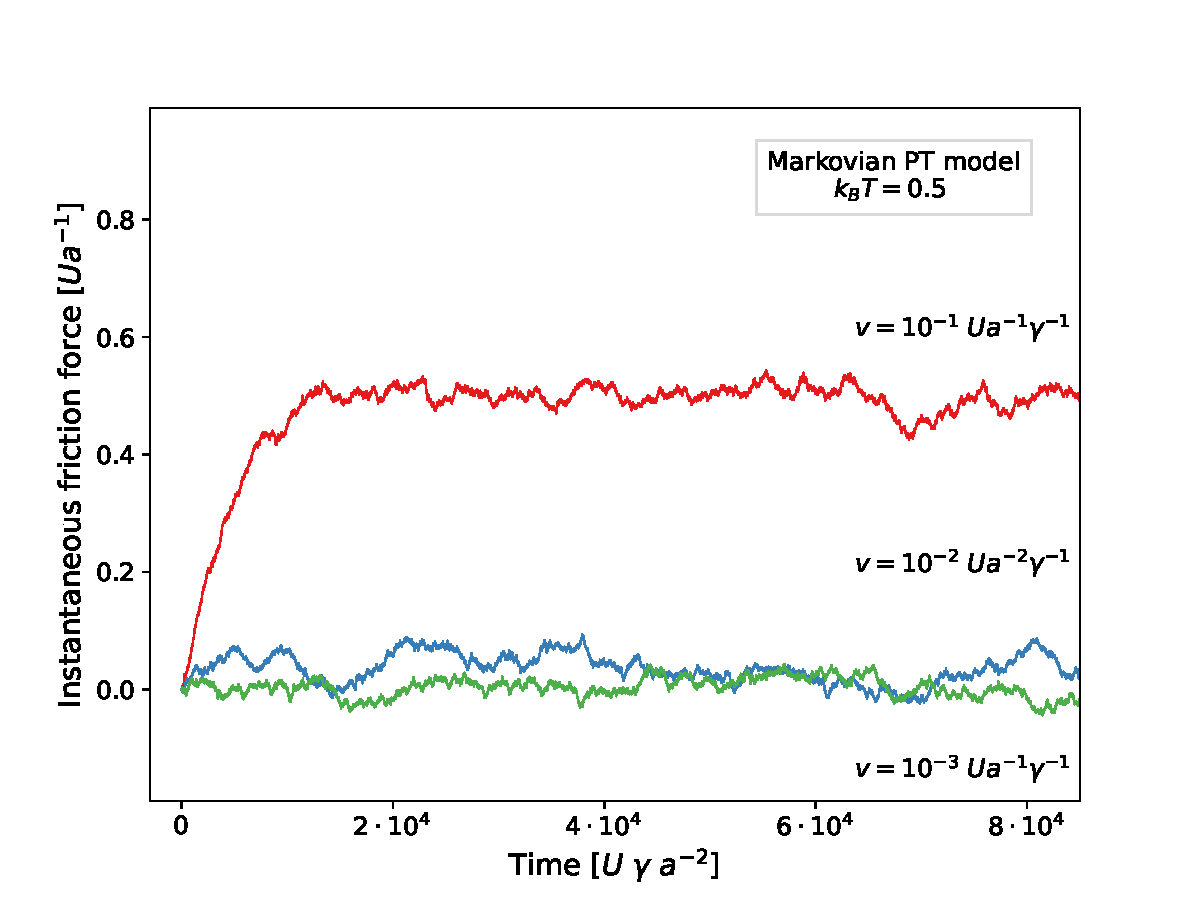
\includegraphics[width=\textwidth]{basseV_kb0_forzaplot.pdf}
    \caption{Friction force as a function of time in the Markovian PT model, in the low-velocity regime }
    \label{fig:basseV_kb0_friction}
\end{figure}
Regarding the velocity-dependence of the friction force in the more interesting low velocity regime, we conduct only a preliminary study is conducted due to subtle difficulties associated to numerical data analysis. Specifically at very low velocity, under $10^{-3}\hspace{0.1cm}U\gamma^{-1} a^{-1}$, the effects of stochastic thermal forces cause the particle to jump from one minimum to another, with the dragging-forward dynamics remaining a minor, perturbative effect. Figure \ref{fig:basseV_kb0_friction} illustrates how already at $v \simeq 10^{-2}\hspace{0.1cm}U\gamma^{-1} a^{-1}$ or $10^{-3}\hspace{0.1cm}U\gamma^{-1} a^{-1}$, the friction force fluctuates widely: these fluctuations are comparable in size to the average friction force itself, or even larger. As a result, extracting a significant friction force from the time average rapidly becomes a formidable task, that would require extremely long simulations to average out the thermal noise.

For $v<0.01\; U\gamma^{-1}a^{-1}$ outlined above where diffusion dominates over driving, we choose to perform a time averaging without omitting any transient, which is not well-defined, and to carry it out over the entire simulation time, which we extend from a minimum $10^6 \hspace{0.1cm}t_0$ up to $2 \cdot 10^7 \hspace{0.1cm}t_0$, depending on the slider velocity. This choice is made for the standard Prandtl-Tomlinson situation, which can be seen in Figure \ref{fig:basseV_kb0_friction}.
\begin{figure}
    \centering
    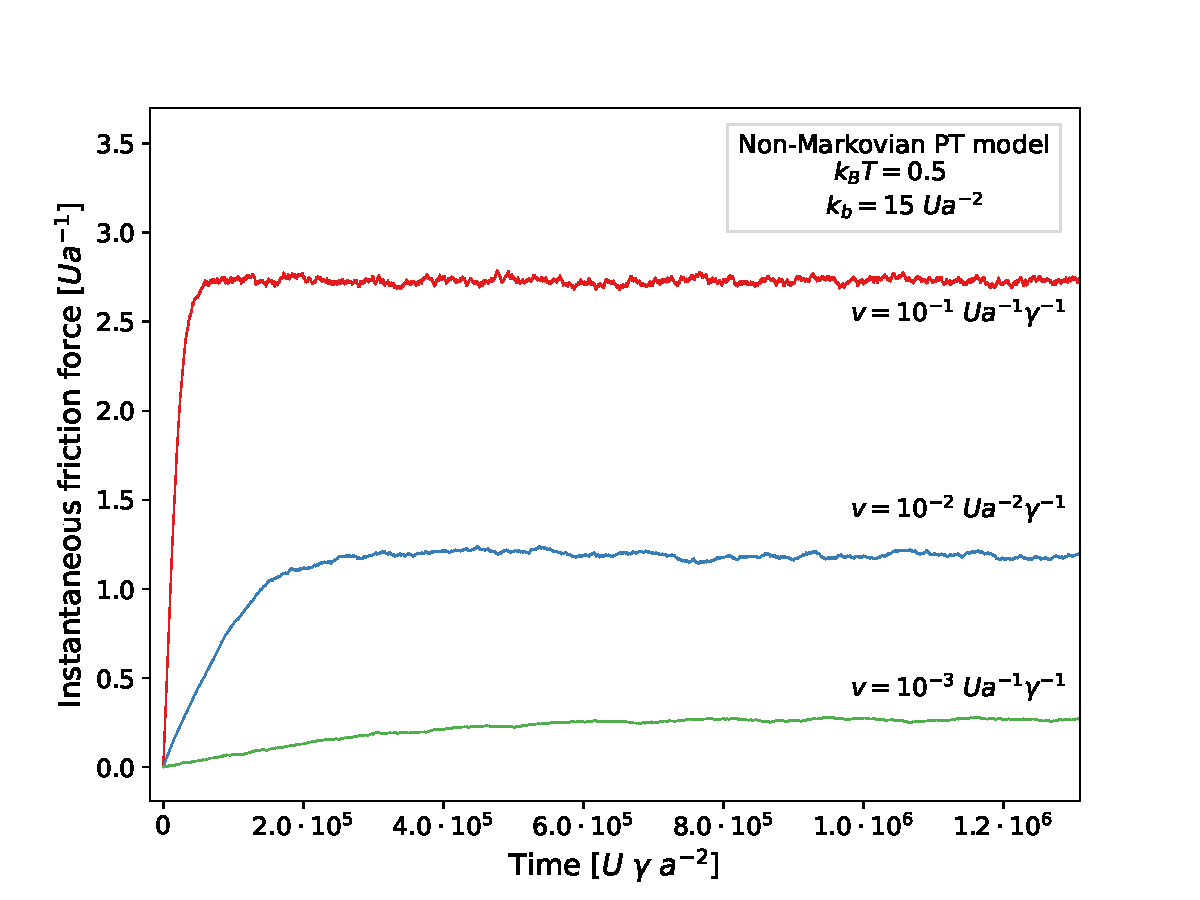
\includegraphics[width=\textwidth]{basseV_kb15_forzaplot.pdf}
    \caption{Friction force as a function of time in the non-Markovian PT model, in low velocity regime.}
    \label{fig:basseV_kb15_friction}
\end{figure}
\\
In the scenario of non-Markovian Prandtl-Tomlinson, Fig. \ref{fig:basseV_kb15_friction}, due to the coupling with a more strongly damped environment, the friction force is more stable over time. This leads to a more reliable and computationally simpler determination of its value even in the low-velocity regime. This figure allows us to appropriately select the transient part to be excluded from the temporal averaging of the friction forces. It is observed that this quantity increases significantly as the velocity decreases, reaching $10^6\hspace{0.1cm}  t_0$ for $v=10^{-3} \hspace{0.1cm} Ua^{-1}\gamma^{-1}$.

Figure \ref{fig:totale_logartimX} compares the velocity dependence of the time-averaged friction force for both the Markovian and non-Markovian PT models as a function of the driving velocity in $\log{(v)}$ scale, across a broad velocity range. This figure also includes the value of the static friction force $F_\text{static}$ calculated in Section \ref{ourmodel}.
\begin{figure}
    \centering
    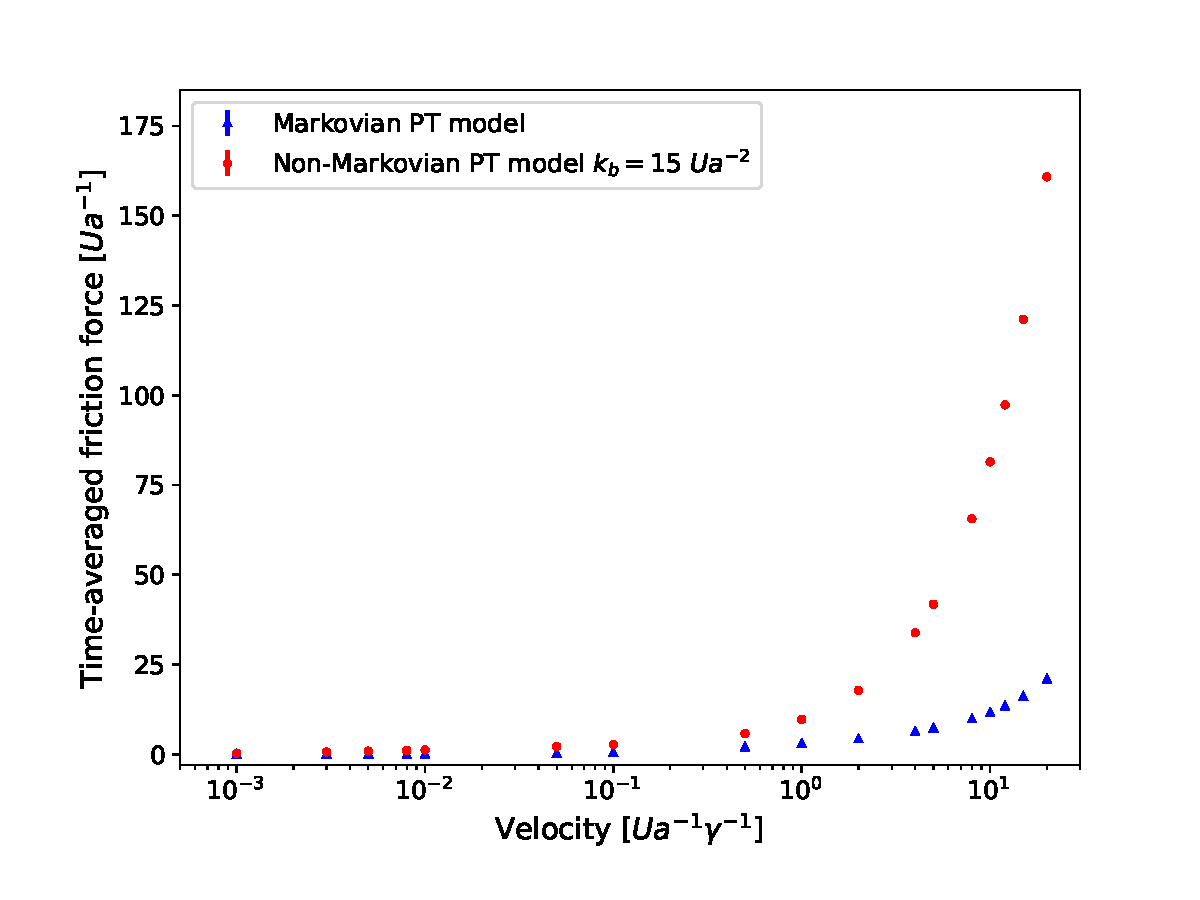
\includegraphics[width=\textwidth]{tot_logaritmica.pdf}
    \caption{Same as Fig.~\ref{fig:high_velo_friction}, but with velocity in logarithmic scale.}
    \label{fig:totale_logartimX}
\end{figure} We observe that in the low-velocity regime, the time-averaged friction force deviates from the linear variation appropriate for large velocity, but exhibits a much slower variation. For the standard PT over a limited range, the expected velocity-dependence is verified (Fig. \ref{fig:low_velocities}) with a curve fit in the following form  
\begin{equation}
    F(v) = f - a \log{\left(\dfrac{b}{v}\right)}^\frac{2}{3}\; ,
\end{equation}
Table \ref{tab:param_lowvel} reports the best-fit parameters.
\begin{table}
\centering
\begin{tabular}{ccc}
    \toprule
    \multicolumn{3}{c}{Fit parameters} \\
    \midrule
   $f$ [$Ua^{-2}$] &  $a$ [$Ua^{-2}$] & $b$ [$Ua^{-1}\gamma^{-1}$] \\
    \midrule 
    $0.03 \pm 0.02$ & $0.05\pm 0.03$ & $0.010 \pm 0.001$ \\
    \bottomrule
\end{tabular}
\caption{Best-fit coefficients for the velocity-dependence of friction force in low-velocity regime.}
\label{tab:param_lowvel}
\end{table}
For the non-Markovian PT model Figure \ref{fig:low_velocities} indicates that it may be necessary to repeat the calculations for smaller velocity $v$ to verify the low-speed behavior of the model.
\begin{figure}
    \centering
    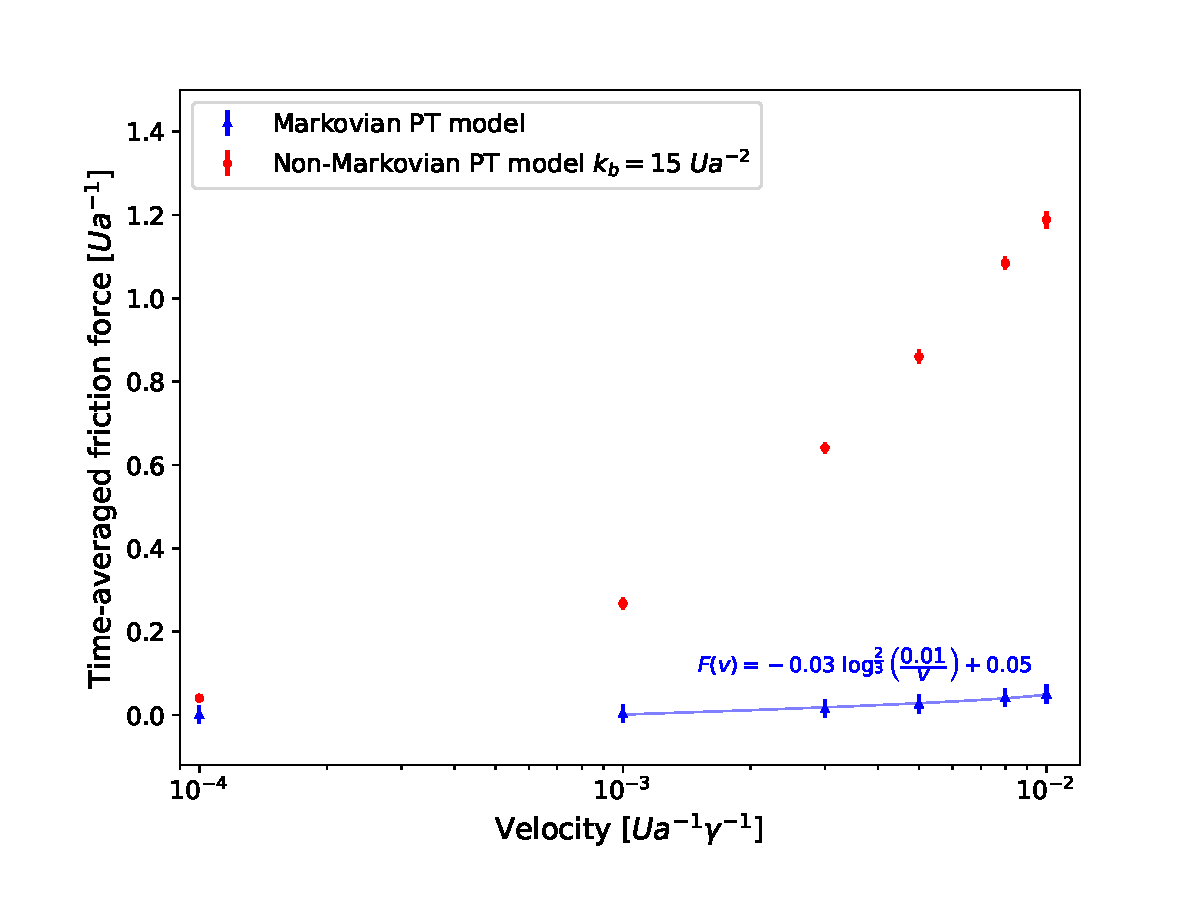
\includegraphics[width=\textwidth]{lowvelocities.pdf}
    \caption{Same as Fig.~\ref{fig:totale_logartimX}, detail of the low-velocity range.}
    \label{fig:low_velocities}
\end{figure}
